\chapter{Introduction}
\label{chapter:intro}
\section{A little motivation}

The desire to infer precise and accurate stellar ages is motivated by a number
of scientific questions.
For example, without this fundamental stellar property, the evolution of stars
and stellar populations would be a mystery.
In addition, our understanding of the formation history of the Milky Way would
be limited and with it, the formation process of all galaxies.
Some day in the (hopefully) not-too-distant future, the first biomarker will
be detected in the atmosphere of an Earth-like planet.
When that time comes, knowing the age of the planetary system will be
fundamental.
These are all excellent reasons for studying stellar ages but the application
that most piques my personal interest is the implications for understanding
the dynamical evolution of exoplanetary systems.

Despite the rapidly accelerating interest in exoplanet population studies
\citep[e.g.][]{Petigura2013, Foreman-Mackey2014, Dressing2015, Burke2015}, we
still know very little about how planetary systems {\it evolve} because
stellar ages are difficult to infer.
Planetary system architectures are not static in time: chaotic gravitational
interactions can fling planets into interstellar space or plunge them into the
surface of their star.
If they cross orbits they can even collide or be excited to highly eccentric
and inclined orbits.
Simulations of planetary systems often demonstrate that planet losses are most
common in the few millions of years immediately after formation and continue
at a gradually decreasing rate \citep[e.g.][]{Zhou2007, Smith2009, Funk2010,
Pu2015}.
Planet-planet scattering on extended timescales may result in a decrease in
exoplanet frequency with stellar host age in the enormous sample of over five
thousand exoplanets discovered to date {\it if} their ages can be sufficiently
constrained \citep{Veras2015}.

Determining the detectability of trends in the ages of \Kepler\ systems is
challenging as the outcomes of simulations depend strongly on input
assumptions---different studies therefore produce different predictions
\citep[see figure 3 of][]{Pu2015}.
However, based on the \citet{Smith2009} simulations of systems with three
Earth-mass planets, \citet{Veras2015} demonstrate that a decrease in planet
occurrence rate will be detectable for K dwarf hosts, even if stellar age
uncertainties are as large as 5 Gyr, and for G dwarfs with age uncertainties of
3.5 Gyr.
Clearly, most systems do not consist of equal-mass planets, but the study
of these simulations demonstrates that an age trend lies well within the
realms of detectability.

This is just one of the tantalising scientific discoveries looming on the
horizon, if only we could improve our methods for inferring precise stellar
ages.
As I explain in this thesis, my research has advanced our understanding of the
stellar age-rotation, or `gyrochronology' relations, contributing to our
ability to infer stellar ages as a community.
This research may ultimately lead to discovering variations in the
architecture and frequency of exoplanets as a function of host star age.


\section{Stellar dating methods}

The hydrogen-burning era of a star's life is extremely stable.
This fact is unfortunate from a stellar chronologist's point of view as,
without an observable property that is a strong function of age, stellar age
precision will always be limited.
This is the main stumbling-block for stellar age inference: age precision is
restricted by the fundamental evolutionary timescale of stars.
Despite this limitation however, there is still plenty of room for progress to
be made in understanding the evolution of the observable properties from both
empirical and theoretical standpoints, and in the precision with which we can
measure these properties.

Isochronal ages are notoriously difficult to infer because stars vary little
in brightness or temperature during their hydrogen-burning lifetimes.
Fitting stellar evolutionary models to these two observables usually produces
age estimates with uncertainties in the order of 50-150\%.
However, because cool stars spin down predictably over their main sequence
lifetime due to magnetic braking, their current rotation periods depend, to
first order, only on their masses and ages.
Photometric measurements of these two parameters can therefore be used to
infer an age.
This is the concept behind `gyrochronology'---inferring an age from a rotation
period---developed after observations of stars in clusters revealed a trend
for decreasing rotation period with time, at a given mass \citep{Weber1967,
Skumanich1972, Barnes2003, Irwin2009}.
This method has never held as much promise as it does now, with a new glut of
stellar rotation periods available from a new generation of spacecraft
designed for high precision, high cadence photometry.
The main science goal of these missions is searching for exoplanets, but the
exoplanet gold-rush has lead to a new understanding of stars and stellar
variability.
The desire to develop a method of dating stars using only photometry is an
understandable one with the current availability of such large photometric
data sets.
However, as with any phenomenological investigation, inferences about the data
can only be made with models.
These models can be physical or empirical but whatever the origin of their
design, they must be calibrated using observations.
No age model can be developed in isolation from the observations---our
understanding of stars just isn't good enough.
So when a new dating method is developed, its efficacy relies on the existence
(and precision) of previous dating methods.
It is therefore important to understand the currently available dating
methods, their advantages and their limitations.
In what follows, I describe the main methods used today.

\subsection{Isochrone fitting}

As stars burn hydrogen they become hotter and more luminous, slowly moving
towards the top right of the Hertzprung-Russel Diagram (HRD), or
Colour-Magnitude Diagram (CMD).
As the hydrogen-burning process progresses, helium `ash' is produced in the
core and energy production decreases.
The core slowly contracts over time and its temperature therefore increases.
The increased temperature enhances energy production, and the result is that
stars burn hotter and more brightly over time.
By inferring a star's absolute magnitude and effective temperature, or
measuring its colour, plus its composition and evolutionary stage, it is
possible to place it on an HRD or CMD and infer its age.

In practice, it is not usually possible to feed luminosity, temperature,
metallicity and \logg\ into a stellar evolution model, crank the handle and
pull out an age.
Evaluating these models is expensive, so pre-calculated model grids are used.
In order to infer an age from the observations it is therefore necessary to
interpolate between grid lines.
The Dartmouth \citep{Dotter2008}, Yonsei-Yale (Y$^2$) \citep{Yi2001,
Spada2013}, Padova \citep{Girardi2002} and PARSEC \citep{Bressan2012} models
are some of the most commonly used sets of models.
These and other isochrone grids compute slightly different ages for the same
star because the underlying stellar evolution models are different.
For example, the four models listed above use different equations of state,
different models for opacity within the stars and different atmospheric
models \citep[see][for a comparison of these four sets of
isochrones]{Thompson2014}.

An obvious limitation of the isochrone method is that the composition of the
star in question will affect its placement on a HRD or CMD: metal-rich stars
appear cooler and redder than metal-poor ones with the same mass and age.
% FIXME: why?
It is often difficult or impossible to obtain precise metallicities, helium
abundances and alpha-element fractions (all needed for precise isochrone
placement), as these measurements come from expensive, high-precision
spectroscopy.
% FIXME: how are these things actually extracted from spectra?
However, for an ensemble of coeval stars with identical compositions this
process becomes much easier: not only are there more opportunities to measure
stellar compositions, providing a $\sqrt N$ reduction in measurement
uncertainty, a group of stars with the same age and composition but different
masses will reveal the shape of the best-fitting isochrone on the CMD\@.
In addition, the position of the main sequence (MS) turn-off further improves
age precision.
Since MS lifetime is strongly dependent on mass, at any given age the most
massive stars in a cluster will have turned off the MS.
Inferring the mass at which this happens in a cluster provides a very precise
age estimate.
% FIXME: what is the minimum age at which you can do this?
For these reasons, many open clusters have precise ages with typical age
uncertainties of around 10\%, arising chiefly from differences in isochrone
models.
Together with the Sun they are the most precisely dated of all astronomical
objects and provide the benchmarks from which all other dating methods are
calibrated.
Figure \ref{fig:hyades} shows 69 field stars in the Hyades plotted on a CMD
from \citet{Perryman1998}.
Isochrones at a range of ages are also shown, as is the Zero Age Main Sequence
(ZAMS), the line upon which stars fall as they enter the main sequence.
\citet{Perryman1998} infer an isochronal age of 625 $\pm$ 50 Myr for the
Hyades.

\begin{figure}[p]
\begin{center}
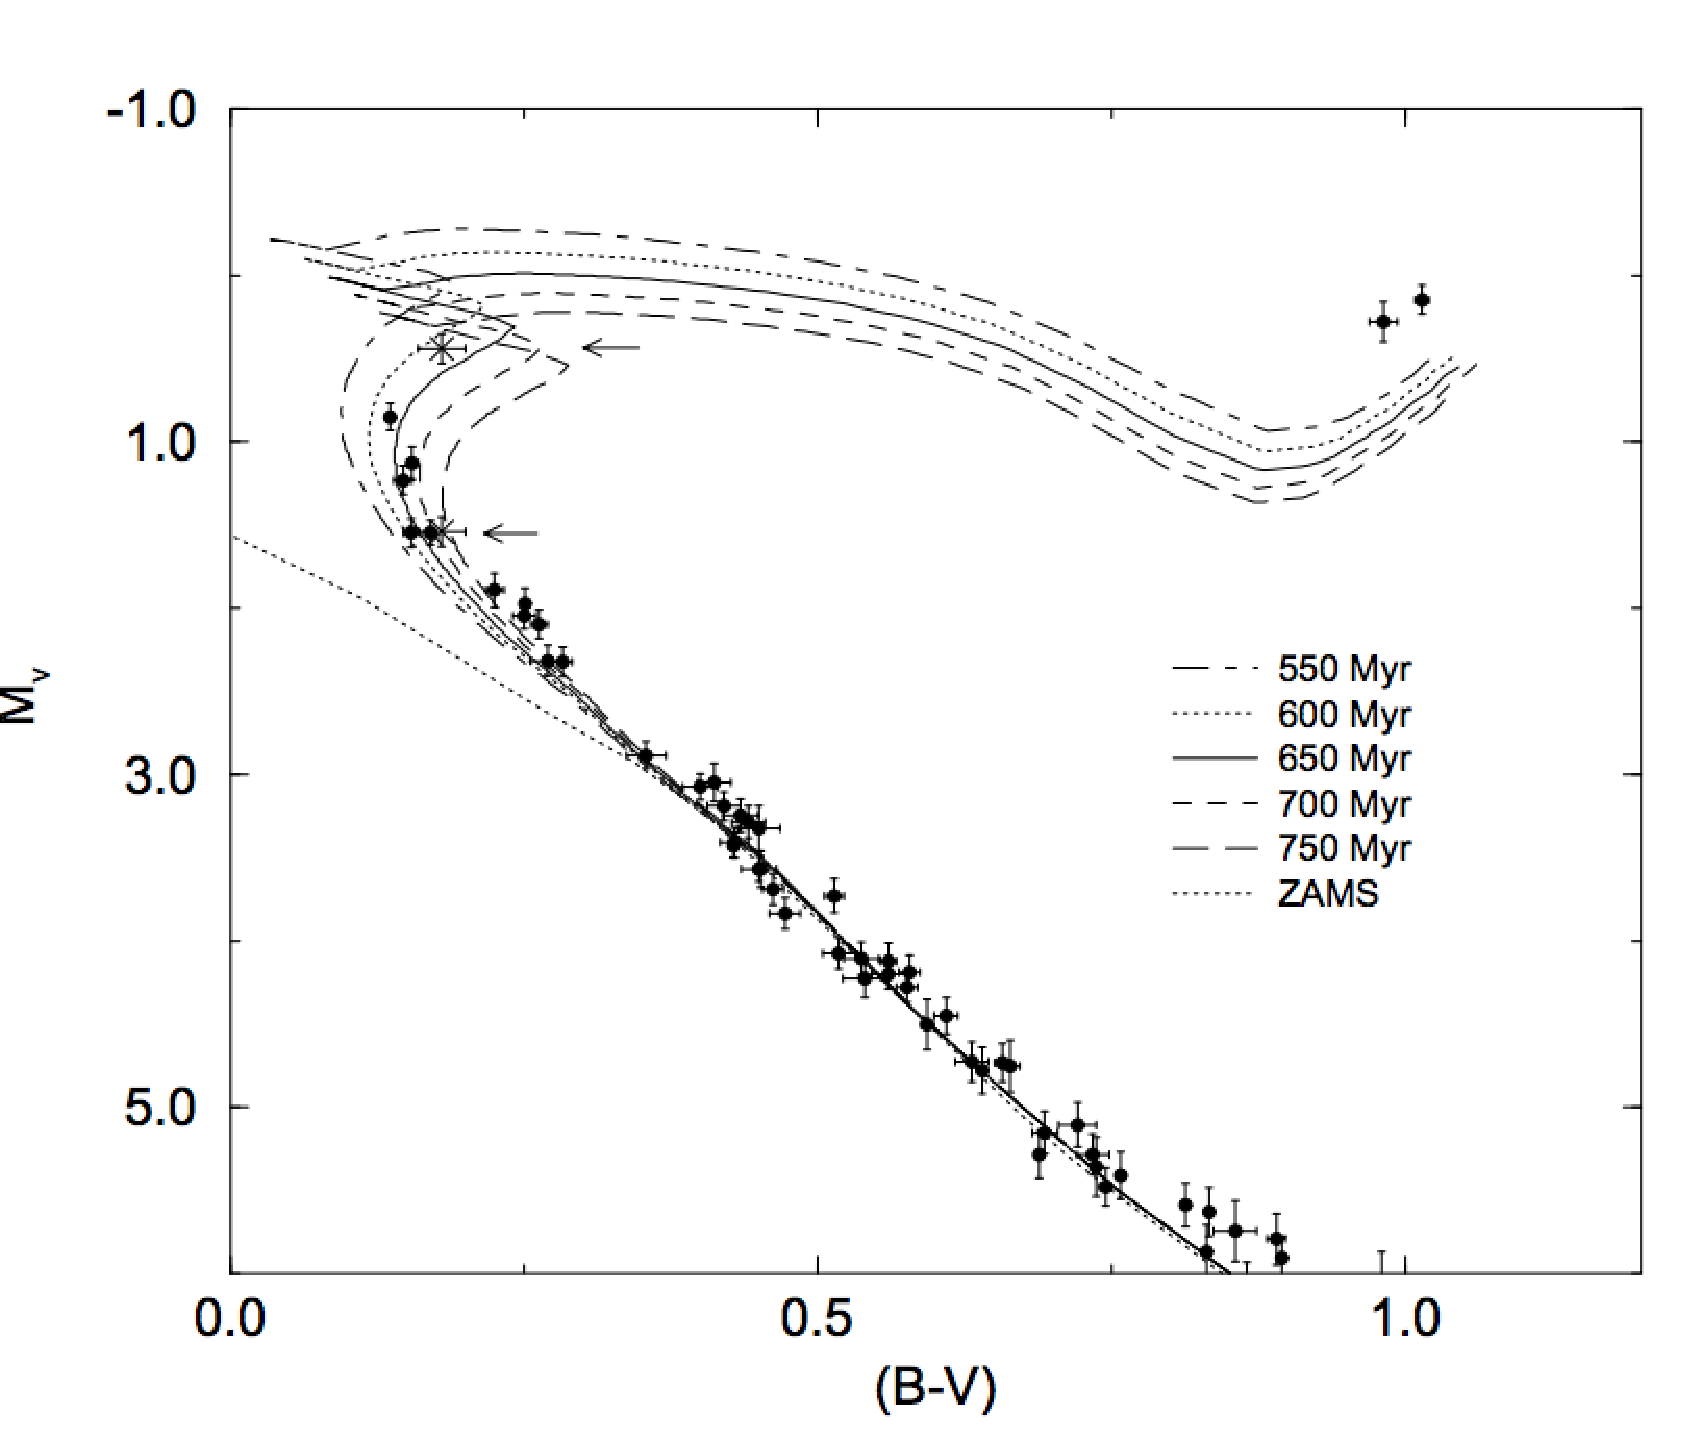
\includegraphics[width=6in, clip=true]{figures/hyades.pdf}
\caption[A CMD of the Hyades.]
{A CMD of the Hyades with Geneva isochrones \citep{Schaller1992} and the ZAMS
from \citet{Perryman1998}.
\citet{Perryman1998} infer an isochronal age of 625 $\pm$ 50 Myr for the
Hyades.}
\label{fig:hyades}
\end{center}
\end{figure}

% For example Pleiades (0.55 Gyr), Hyades (0.625 Gyr), Praesepe (0.588 Gyr), and
% Coma Berenices (0.5 Gyr).
% Download isochrones and estimate the ages of some KOIs.

\subsection{Asteroseismology}
\label{sec:asteroseismology}

The NASA \kepler\ mission plays a fundamental role in this thesis.
I describe the \kepler\ space craft and its unique data set in detail in
\textsection \ref{sec:kepler}.
The main objective of the \kepler\ mission is to search for extra solar
planets using the transiting method, however since extremely precise
photometry is required for exoplanet search, a number of other scientific
fields have benefited from its exquisite light curves.
\kepler's legacy is not limited to exoplanets---it has arguably advanced
stellar astronomy more than any other single purpose astronomical instrument
ever created.
Among its several successes is the improvement of stellar dating methods, as
I explain below.

After exoplanet search, arguably the second most important branch of \kepler's
legacy is asteroseismology; the study of stellar pulsations.
% QUESTION: difference between solar and classical pulsations?
% ANSWER: Solar are small enough that you can maintain certain approximations.
Sound waves ripple through the deep interiors of stars.
The frequencies of these waves can reveal internal structure, even localising
the age-dependent hydrogen burning region.
Asteroseismology is a powerful tool in the stellar dating arsenal and while it
is not the central topic of my thesis, it features at some level in almost
every chapter, so I cover the basic principles below.

Acoustic oscillations in the Sun are generated by turbulent convection near
the surface.
The movement of ionized gas stochastically excites the Sun's spherical
oscillation modes.
An analogy to this process is that of a bell in a room filled with air.
Air particles colliding with the surface of the bell cause it to vibrate at
all of its spherical harmonic frequencies.
There is no coherent driving force, rather the stochastic collisions of air
particles induce a continual ringing.
Similarly, the Sun is continually oscillating at a range of discrete
frequencies; those that correspond to its spherical harmonics.
The restoring force of these acoustic oscillations is pressure, thus these
waves are called `pressure' or `p'-modes.
A power spectrum of the Sun, taken from \citet{Brown2000} is shown in figure
~\ref{fig:solar_spectrum}.
The comb-like, evenly spaced peaks in this power spectrum show Solar p-mode
oscillations.
The peak amplitudes are modulated by a Gaussian envelope and the mean of that
Gaussian, $\nu_{max}$ corresponds to a frequency of around 3000 \uHz, a period
of around five minutes.

\begin{figure}[p]
\begin{center}
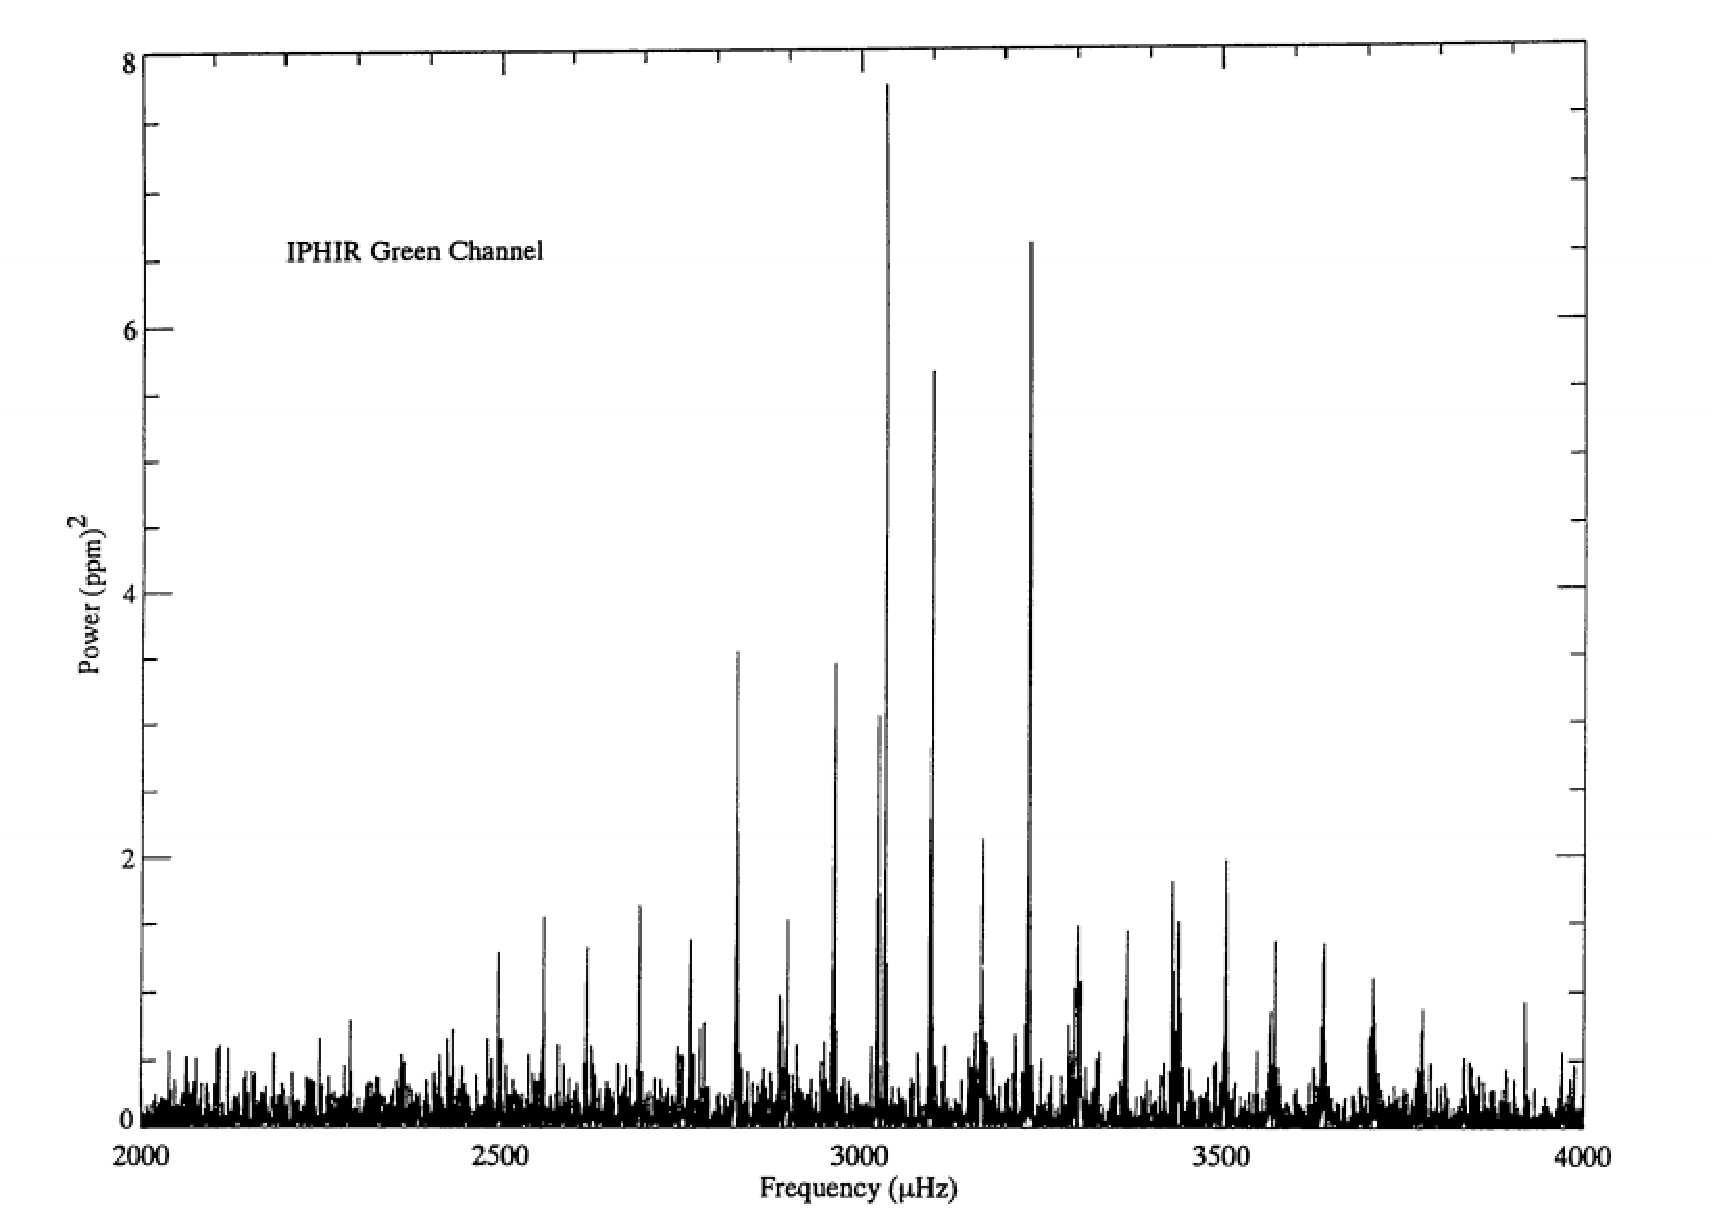
\includegraphics[width=6in, clip=true]{figures/solar_spectrum.pdf}
\caption[Solar power spectrum.]{A power spectrum of one month of
disc-integrated Solar photometry, taken from \citet{Toutain1992}.
Solar p-modes are clearly visible in this figure.}
\label{fig:solar_spectrum}
\end{center}
\end{figure}

Many properties of the Sun have been measured using asteroseismic pulsations,
for example the variation in radial pressure, the rate of differential
rotation, the depth and fraction of helium in its convective zone and even the
structure of active regions below the Solar surface.
The Sun is an exquisite example of a pulsating star, having tens of millions
of detectable modes and mode lifetimes that are several thousand times longer
than the periods of the oscillations.
These long mode lifetimes result in narrow peaks in the Fourier transform of a
Solar light curve or RV time series.
Short-lived modes produce signals that are incoherent over long timescales and
therefore have broadened peaks in frequency space.
Its proximity, which provides both enormous S/N and allows us to resolve the
surface, makes it a paragon of seismology.

Three types of oscillations manifest themselves in stars: pressure (p-modes),
surface (s-modes) and gravity (g-modes).
Pressure provides the restoring force for p-mode oscillations, and these are
effectively sound waves.
Surface modes are, as the name suggests, waves on the surface of the star.
% Since it is only possible to detect s-mode waves if the stellar surface is
% resolvable, this type of wave has only been seen in our Sun.
G-modes are excited by buoyant gas in the radiative zone and the restoring
force is gravity.
G-mode waves rapidly evanesce in stellar convective zones and therefore
appear at very low amplitudes at the surface of Sun-like stars.
For the work in this thesis I am concerned only with p-mode observations as
these waves reveal the internal structure of a star which varies as a function
of mass, radius and age.

The frequency of a p-mode wave is proportional to the sound-speed of the gas
along its path through the stellar interior.
Time-dependent spatial perturbations to a star's equilibrium state can be
written as a product of a term that depends on stellar radius and a spherical
harmonic (assuming that a star can be approximated as a sphere) as follows
\citep{Brown1994},
\begin{equation}
    \xi_{nlm}(r, \theta, \phi, t) = \xi_{nl}(r)Y_l^m(\theta, \
    \phi)e^{-i\omega_{nlm}t}.
\end{equation}
$\xi$ is a spatial perturbation, associated with a mode, $r, \theta, \phi,
\omega$ and $t$ are the radial coordinate, colatitude, longitude angular
frequency\footnote{The convention in asteroseismology is to report circular
frequencies, $\nu_{nlm} = \omega_{nlm}/2\pi$.} and time, respectively.
$n$ is the radial order, defined as the number of nodes between the star's
centre and surface and $l$ is the angular degree, the product of the stellar
radius and the total horizontal wavenumber of the mode.
For example, a star oscillating with an $l = 10$ mode will have a standing
wave with 10 nodes along a line connecting the poles.
Finally, $m$ is the azimuthal order; the projection of $l$ onto the horizontal
wavenumber of mode and must be less than or equal to $l$.
A star with an $m = 5$ mode will have a standing wave with 5 nodes along the
equator.
The relation between $\omega$ and $n$ and $l$ is complicated and depends on the
structure of the star.
Oscillations with different values of $l$ penetrate to different depths in the
star.
$l = 0$ waves travel through the centre and waves with increasing $l$ skirt
the central region by a larger and larger distance.
For this reason, modes with different $l$ provide information about the sound
speed gradient in the stellar interior.
The `small frequency separation', $\delta_{n,l} = \nu_{n+1, l} - \nu_{n, l+2}$
is often used to parameterise the variation in frequency with stellar radius
via \citep{Brown1994}
\begin{equation}
    \delta_{n,l} = \Delta\nu_0\frac{(l + 1)}{2\pi^2\nu_{nl}}\int_0^{R_\star}
    \frac{dc}{dr}\frac{dr}{r}.
\end{equation}
Since nuclear-burning material in the core changes its molecular weight as the
star evolves, the sound-speed gradient is time-dependent and the small
separation therefore contains information about the age of the star.

There is no simple harmonic relation between the frequencies of modes with
adjacent mode number \citep{Brown1994}.
% check this!
However, in the limit where $n \gg l$, mode frequency can be approximated as
\begin{equation}
    \nu_{nl} = \Delta\nu_0\left(n + \frac{l}{2} + \epsilon \right) - \
    \frac{AL^2 - \eta}{(n + l/2 + \eta)},
\end{equation}
where parameters $\Delta\nu_0$, $A$, $\epsilon$ and $\eta$ depend on the
structure of the star and $L^2 = l(l+1)$.
$\Delta\nu_0$ is the `large frequency separation' which, together with the
peak frequency of the Gaussian envelope that modulates the amplitudes of the
oscillation modes, $\nu_{max}$, makes up the two fundamental asteroseismic
observables.
It is related to the sound travel time through the centre of the star:
\begin{equation}
\Delta\nu_0 = \left(2\int_0^{R_\star}\frac{dr}{c}\right)^{-1},
\end{equation}
where $c$ is the local sound speed and $R_\star$ is the stellar radius.
This travel time is related to the mean density of the star via,
\begin{equation}
\Delta\nu_0 \cong 135\left(\frac{M_\star}{R_\star^3}\right)^{1/2}\mu Hz,
\end{equation}
where $M_\star$ and $R_\star$ are the stellar mass and radius in Solar units
\citep{Cox1980, Brown2000}.

Today, p-modes have been detected in hundreds of Sun-like stars, however it
was not until the late 1990s that the first conclusive detection was made in
a star other than our Sun.
The reason for this is simply that p-mode perturbations are extremely
small---these changes are around 10 cms$^{-1}$ in velocity and 3$\mu$mag in
brightness for typical oscillation modes in the Sun \citep{Brown2000}.
Asteroseismic pulsations are usually detected in two different ways: by
searching for the subtle change in luminosity caused by the temperature
fluctuations of the stellar surface, or by measuring the changing radial
velocity of the surface.
A Fourier transform of these time series will reveal the presence of
oscillation modes, allowing for the modelling of the star's interior
structure.
The earliest p-modes detections were made using radial velocity data
\citep{Kjeldsen2001} for stars $\eta$ {\bf Boo} \citep{Kjeldsen1995}, {\bf
Procyon} \citep{Barban1999, Martic1999}, $\zeta$ {\bf Herculis}
\citep{Martic2001}, $\alpha$ {\bf Cen A} \citep{Kjeldsen1999} and $\beta$ {\bf
Hyi} \citep{Bedding2001}.
Today, we can take advantage of space-based missions \kepler\ and \corot\
whose photometric precision provides sufficient S/N to detect
p-mode-induced luminosity variations.
These missions have provided fundamental parameters for hundreds of
oscillating giants, subgiants and Sun-like stars \citep[e.g.][]{Michel2008,
Bruntt2009, Chaplin2014}.

% In the previous section I describe the relations between stellar p-mode
% oscillation frequencies and the physical parameters of a star.
% In this section I will describe the application of asteroseismology: how
% exactly does one infer fundamental stellar parameters from a light curve?
% My thesis work focuses on \kepler\ data, so this discussion will be directly
% related to \kepler\ data, but the same principles apply to other photometric
% time series.

The frequencies of oscillations accessible in \kepler\ light curves are
limited by two things: the overall duration of observations and the time
sampling interval.
The duration of observations, \ie\ the length of the \kepler\ mission sets the
minimum resolvable frequency and the time sampling sets the Nyquist frequency:
the high frequency limit, which is equal to half the sampling rate.
For FGK dwarfs, the Nyquist frequency of long cadence observations ($\sim 283
\mu$Hz) is too low as these stars oscillate at around 3000 \uHz.
For this reason, \kepler\ operates in two observing modes: long and short
cadence.
Long cadence observations are taken approximately every 30 minutes and short
cadence every minute ($\nu_{Nyquist} \sim 8333$\uHz).
Around 560 dwarfs and subgiants were observed in short cadence mode
\citep{Chaplin2014}.

There are two different approaches to inferring asteroseismic ages from
\kepler\ light curves, depending on the signal-to-noise ratio (S/N) of
pulsations.
In the high S/N cases it may be possible to identify
oscillation frequencies of individual modes \citep[\eg][]{Metcalfe2010,
Silva-aguirre2012, Lebreton2014}.
However for the majority of short cadence targets, only the
mean large frequency separation, $\Delta\nu$ and frequency of maximum power,
$\nu_{max}$ can be measured.
Bulk physical properties of stars can be inferred from these two parameters
via the scaling relations \citep{Brown1991, Kjeldsen1995}:
\begin{equation}
    \frac{M}{M_\odot} = \left(\frac{\nu_{max}}{\nu_{max,\odot}}\right)^3
    \left(\frac{\Delta\nu}{\Delta\nu_\odot}\right)^{-4}
    \left(\frac{T_{\mathrm{eff}}}{T_{\mathrm{eff},\odot}}\right)^{3/2}
\end{equation}
\begin{equation}
    \frac{R}{R_\odot} = \left(\frac{\nu_{max}}{\nu_{max,\odot}}\right)
    \left(\frac{\Delta\nu}{\Delta\nu_\odot}\right)^{-2}
    \left(\frac{T_{\mathrm{eff}}}{T_{\mathrm{eff},\odot}}\right)^{1/2}.
\end{equation}
These scaling relations have been tested on Solar-like oscillators and give
good agreement with the observations \citep[\eg][]{Chaplin2013, Coelho2015}.
Ages are then inferred by comparing these quantities to those predicted by
model grids (spectroscopic estimates of \teff\ and \feh\ are also required).
Two of the most sophisticated codes used for age analysis are the BAyesian
STellar Algorithm \citep[BASTA][]{Silva-aguirre2015} and the Bellaterra
Stellar Properties Pipeline \citep{Serenelli2013}.
Ages inferred using \dnu\ and \numax\ typically have relatively large
uncertainties, in the order of 15-40\% \citep{Silva-aguirre2015a}.
In high S/N cases, ages are inferred by adjusting the parameters of stellar
interior models \citep[\eg][]{Kjeldsen2008} until the observed frequencies, or
combinations of them are reproduced.
Uncertainties on ages inferred from high S/N light curves using this
`boutique' method of modelling individual frequencies are typically around
10-15\% \citep{Silva-aguirre2015a}.

Asteroseismology is a powerful dating method with the potential to yield
extremely precise stellar ages.
However, the era of asteroseismology has only just arrived and this fledgling
field is still only applicable to a small number of extremely bright stars
observed by precise photometric space-missions.
Given the quantity of up-and-coming photometric space missions,
asteroseismology will continue to provide precise stellar parameters for
decades to come.
However, accurate and precise asteroseismic ages demand high-precision
photometry of bright (brighter than around 12th magnitude) stars.
Even with \kepler\ and \corot, this only amounts to around one hundred MS
stars with asteroseismic ages available today.
It is therefore essential that alternative dating methods, which can be
applicable to a much larger sample of stars, are developed; age-rotation
relations, for example.

\subsection{Age-rotation relations}

Asteroseismology is revolutionising stellar astronomy and, perhaps in
particular, stellar ages (partly because the bar is so low to begin with).
However, the quantity of ultra-precise, short cadence light curves is limited
and it is still a `by hand' method applied to hand-picked, bright, text-book
Solar-like oscillators.
In order to produce a catalogue of stellar ages large enough to be useful for
stellar population studies, we need a method that can be applied to thousands
of stars.
Such a method should require inexpensive observables, be computationally cheap
and be easily automated.
Gyrochronology has the potential to satisfy these criteria.

\subsubsection{Gyrochronology: the theory}

Today, we know that angular momentum loss in main sequence stars is caused by
a magnetised stellar wind \citep{Schatzman1962, Weber1967, Mestel1984}.
The stellar wind is composed of charged ions that stream away from the stellar
surface.
Each of these ions carries mass, charge and angular momentum as it travels
away from the star.
The angular momentum carried by these particles is lost from the system, not
at the photosphere because the wind particles travel along magnetic field
lines which are radial close to the surface of the star (in the corotating
frame), but further away from the photosphere, as thermal expansion slowly
begins to dominate the motion of stellar wind particles.
% Stellar magnetic fields force the particles in the stellar wind to rotate with
% the same angular velocity as the surface, out to the Alfv{\'e}n radius.
% The Alfv{\'e}n radius is the point at which a particle experiences equal force
% from the magnetic field and radiation pressure.
% The Alfv{\'e}n radius can be expressed as \citep{Rosswog2011}
% \begin{equation}
% r_A = \left( \frac{\mu^4}{2GM\dot{M}^2} \right)^{1/7}.
% \end{equation}
% Once beyond the Alfv{\'e}n radius, the particles' angular momentum is lost
% from the star.
This mechanism is the main reason why the rotation periods of stars decay
during their stint on the MS.
In addition, the stellar wind carries mass away from the star and its
internal structure changes due to core hydrogen burning.
Both of these processes alter the star's moment of inertia, however this has
a small effect on rotation period evolution.
Stellar magnetism is almost entirely responsible for rotational evolution on
the main sequence.

The motion of turbulent plasma in the outer layers of low-mass stars drives
the production of a magnetic field \citep[][]{Schatzman1962}.
% FIXME: how does rotation drive the dynamo?
Dynamo theory predicts that this field is then amplified by rotation and
differential rotation \citep[\eg][]{Parker1970}.
Convective turbulence, combined with stellar rotation produces the large-scale
magnetic fields that lock the stellar wind to the star
\citep[\eg][]{Charbonneau2010}.
Rotation period influences magnetic field strength: more rapid rotators have
stronger magnetic fields.
% FIXME: CITATION
The relation between angular momentum loss rate and angular velocity is a
power-law, where the exponent depends on the magnetic field geometry
\citep{Mestel1984, Kawaler1988}.
Magnetic field strength controls the rate of angular momentum loss: a stronger
magnetic field leads to stellar wind particles corotating with the photosphere
out to a greater radius which increases the angular momentum lost per unit
time.
Increasing the mass loss rate and temperature of the stellar wind also results
in an increased angular momentum loss rate, although these have secondary
effects.
% There is a saturation point however, angular momentum loss rate only increases
% with magnetic field strength up to a point \citet{Chaboyer1995, Sills2000}.
For this reason the rate of angular momentum loss is not constant: as a star
loses angular momentum its rotation period decays, as does its magnetic field
strength, so the rate of angular momentum loss decreases.
The overall effect of this process is to force stellar rotation periods to
converge.
% \citet{Reiners2012} showed that angular momentum evolution is a function of
Rapid rotators experience a greater angular momentum loss rate than slower
rotators.
Their rotation periods therefore decay more rapidly than slow rotators and,
after a few hundred million years all low-mass stars appear to rotate at a
rate that depends, to first order, only on their age and mass.

This convergence happens more quickly for early-type stars than late-type.
Whilst F, G and K-type stars may have converged by 500 million years,
\citep{Radick1987, Irwin2009} late M dwarfs may not converge within a Hubble
time.
Since the magnetic dynamo is believed to be generated in the convective zone,
stars with a thin convective layer have a weaker magnetic field.
For this reason they lose angular momentum more slowly.
Angular momentum loss rate therefore varies as a function of stellar mass and
fully radiative stars do not spin down appreciably over their MS lifetime
\citep{Noyes1984b}.
The rotational evolution of fully convective stars is still unknown, however
it is an active field of interest \citep[\eg][]{Mcquillan2013, Newton2015}.

\citet{Weber1967}, \citet{Mestel1987} and \citet{Kawaler1988} developed the first physical model of a star undergoing
magnetic braking.
Since this original work, several theoretically motivated gyrochronology
models have been developed by different groups.
For example, \citet{Collier-cameron1994, Reiners2012, Vansaders2013,
Epstein2014} all draw on the principles laid down by \citet{Kawaler1988}, to
create physical models of rotating stars with magnetic fields, where the rate
of angular momentum loss is related to the rotation period and field strength,
and evolve those stars forward in time.
Although these models are based on the physical processes at play, they must
still be calibrated using observations.
For example, the \citet{Kawaler1988} expression, assuming a linear dynamo is
\begin{equation}
\frac{dJ}{dt} = -K_w\Omega^3\left(\frac{R}{R_\odot}\right)^{0.5}
\left(\frac{M}{M_\odot}\right)^{-0.5},
\end{equation}
where $J$ is angular momentum, $R$ and $M$ are radius and mass respectively
and $K_w$ is a constant that must be calibrated so that the Sun has Solar
rotation at Solar age.
See \citet{Barnes2010b} for a discussion on the various adaptations of this
braking law.
\citet{Vansaders2013} use the following model to describe the rotation period
distribution of cool field stars:
\begin{equation}
\frac{dJ}{dt} = \left\{
                \begin{array}{ll}
                  f_K K_M \omega \left( \frac{\omega_{crit}}{\omega_\odot}
                  \right)^2, \omega_{crit} \leq \omega
                  \frac{\tau_{c}}{\tau_{c, \odot}} \\
                  f_K K_M \omega \left( \frac{\omega\tau_{c}}
                  {\omega_\odot\tau_{c, \odot}}
                  \right)^2, \omega_{crit} > \omega
                  \frac{\tau_{c}}{\tau_{c, \odot}}
                \end{array}
              \right.
\end{equation}
\label{eq:vansaders}
With
\begin{equation}
    \frac{K_M}{K_{M, \odot}} = \left(\frac{R}{R_\odot}^{3.1}\right)
    \left(\frac{M}{M_\odot}\right)^{-0.22}
    \left(\frac{L}{L_\odot}\right)^{0.56}
    \left(\frac{P_{phot}}{P_{phot, \odot}}\right)^{0.44},
\end{equation}
\label{eq:vansaders2}
where $f_K$ is a constant, scaled to produce solar rotation at solar age for
the Sun and $P_{phot}$ is the pressure at the photosphere.
$\tau_c$ is the convective overturn time at the base of the convective zone
$P_{rot}/\tau_c$ is known as the Rossby number, $Ro$.
It is dependent on spectral type and for this reason many people argue that
Rossby number is directly related to the surface magnetic field strength and a
more natural quantity to correlate with age and activity than rotation period
\citep[\eg][]{Vansaders2016} \citep[although this view is not universally
held --- see, \eg][]{Reiners2014}.
This is one of the more recently developed theoretical gyrochronology
relations --- however, as revealed in chapter \ref{chapter:conclusions}, this
equation has now been adapted to describe the most recent observations.

\subsubsection{Gyrochronology: the observations}

\citet{Skumanich1972} provided one of the first indications that stellar
rotation periods decay over time and demonstrated that rotation period,
lithium abundance and chromospheric activity decay is proportional to the
square-root of age.
In figure \ref{fig:skumanich}, equatorial rotational velocity\footnote{ Only
the equatorial velocities of the G stars in the two clusters are indicated.}
versus time (triangles) is plotted on the same axes as lithium abundance
(crosses) and Ca$^+$ emission (circles) for the Hyades and Pleiades clusters,
as well as the Sun.
The Sun is the far right point for each age indicator.
Ursa Major stars are included on the Ca$^+$ emission scale.
Lithium abundance and Ca$^+$ emission were previously known age indicators
(see \textsection \ref{sec:activity}) and this work demonstrated that rotation
period was also related to age.
\begin{figure}
\begin{center}
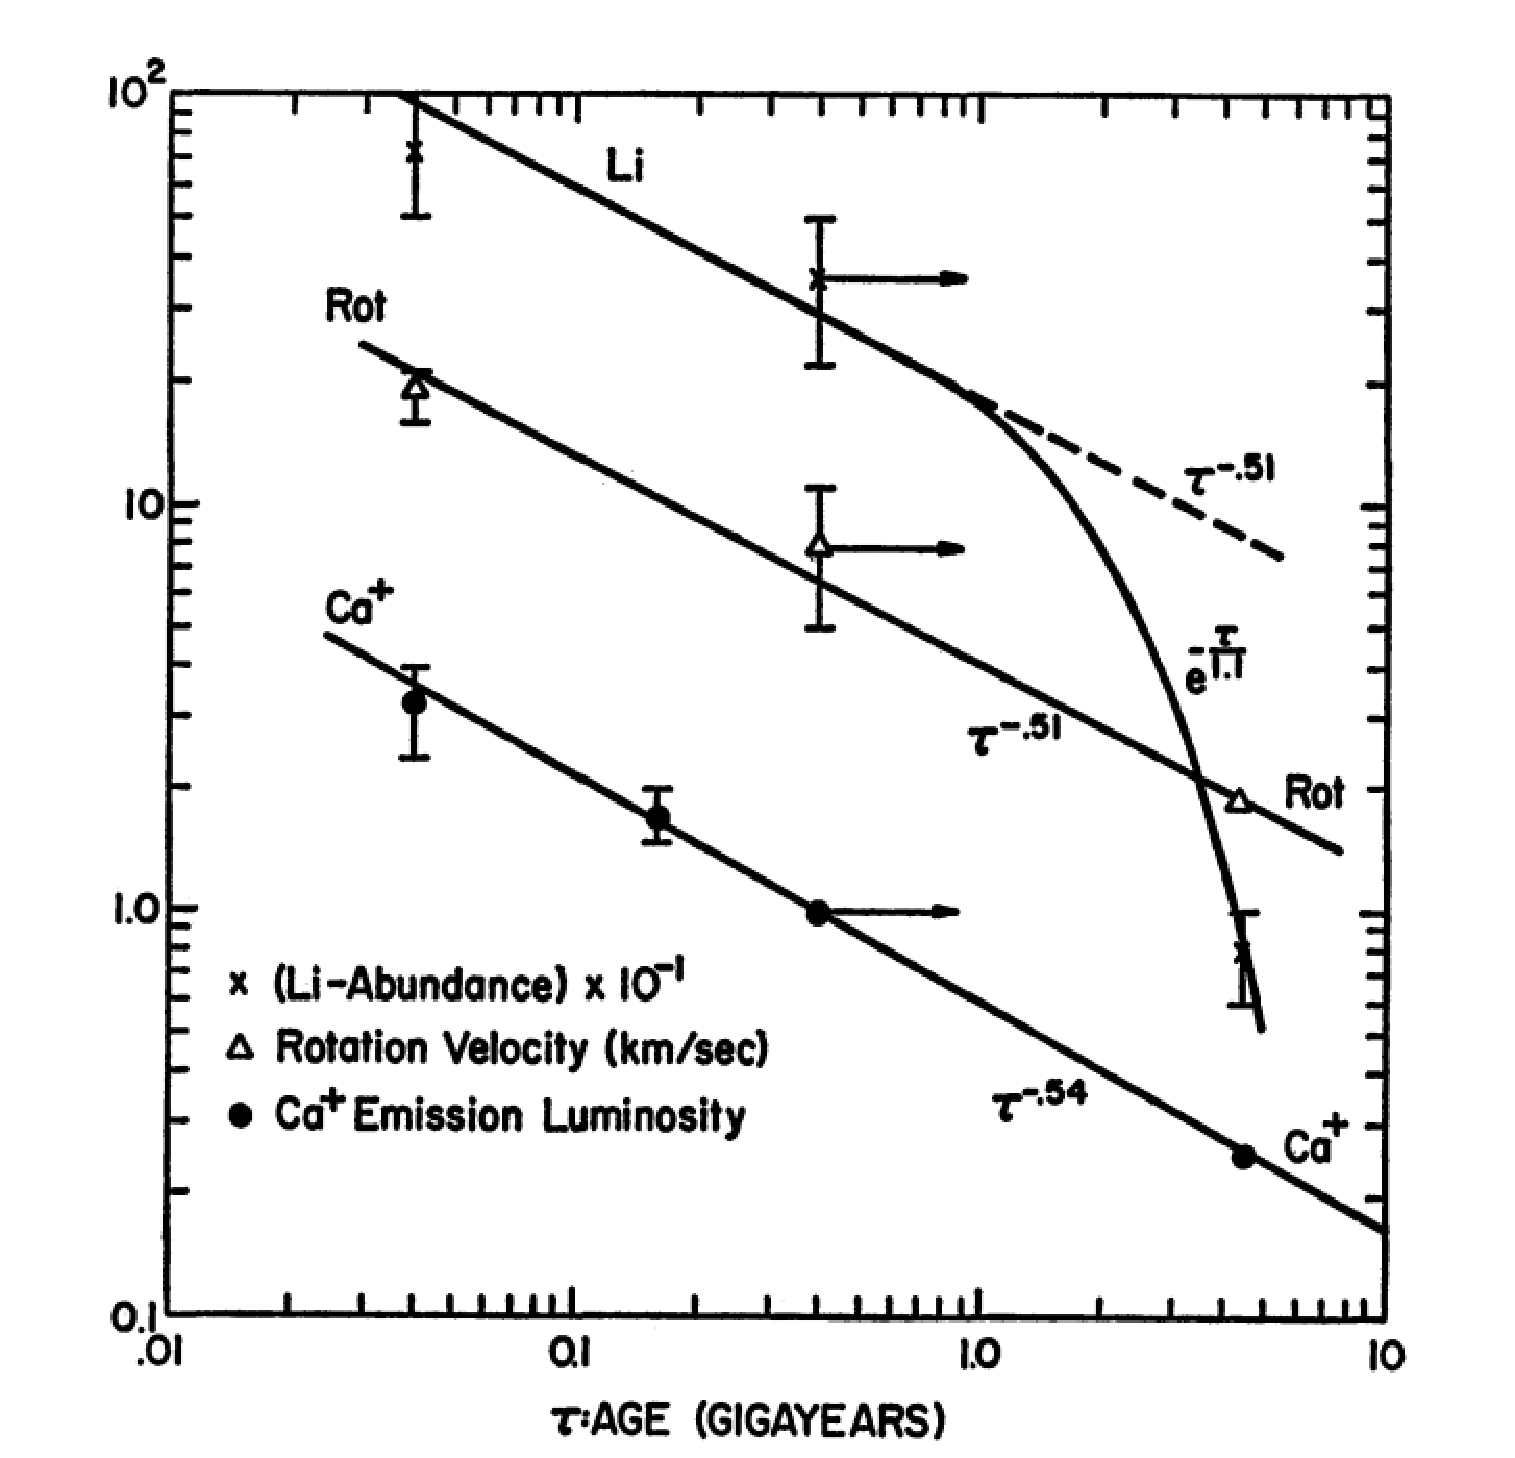
\includegraphics[width=3in, clip=true]{figures/skumanich.pdf}
\caption[\citet{Skumanich1972} results: early evidence for magnetic braking]
{Figure from \citet{Skumanich1972}. Rotation periods for the G stars in the
Hyades and Pleiades and the Sun are plotted.}
\label{fig:skumanich}
\end{center}
\end{figure}

% The rotation periods of cluster stars were investigated in several studies
% \citep[\eg][]{Stauffer1987}.
% The physical mechanism behind the coupling of stellar winds to the magnetic
% dynamo was explored by \citet{Weber1967, Mestel1984}.
% This process was later applied to evolving stars by \citet{Kawaler1988}.

\citet{Kawaler1989} applied the \citet{Kawaler1988} magnetic braking law to
stars in the Hyades cluster and found good agreement with the model.
\citet{Barnes2003} compiled rotation period measurements from members of
several young clusters, plus the Mt. Wilson stars.
% (CITATION)
When the rotation periods of this sample were plotted against B-V colour,
\citet{Barnes2003} noticed that there were two morphological features of the
data (see their figure 2).
In each cluster there was a sequence of stars falling neatly on the predicted
relation between rotation period and mass (called interface or `I' stars),
but there was also a group of rapid rotators (called convective, `C' stars).
The C sequence was most obvious in the younger clusters and less so in the
older.
\citet{Barnes2003} attributed this behaviour to an evolving magnetic dynamo
produced by the still evolving internal structure of the young stars, and
postulated that stars transition rapidly from C to I.
In this work I will only address stars that have already (in theory)
transitioned from the C sequence to the I sequence as they are older than the
Hyades which is the oldest cluster to show this behaviour.

\citet{Irwin2009} compiled rotation period measurements for stars in open
clusters with masses $< 1.2 M_\odot$, shown in figure \ref{fig:irwin}.
These data show the enormous spread in rotation periods for the youngest
clusters (top left), contrasted with the extremely well-defined rotational
sequence in the Hyades (second panel from the bottom on the right).
The currently accepted view is that after the age of the Hyades, stellar
rotation periods lie on this converged sequence.
When applying gyrochronology to stars younger than this age, the I and C
sequences must be modelled separately.
\begin{figure}[p]
\begin{center}
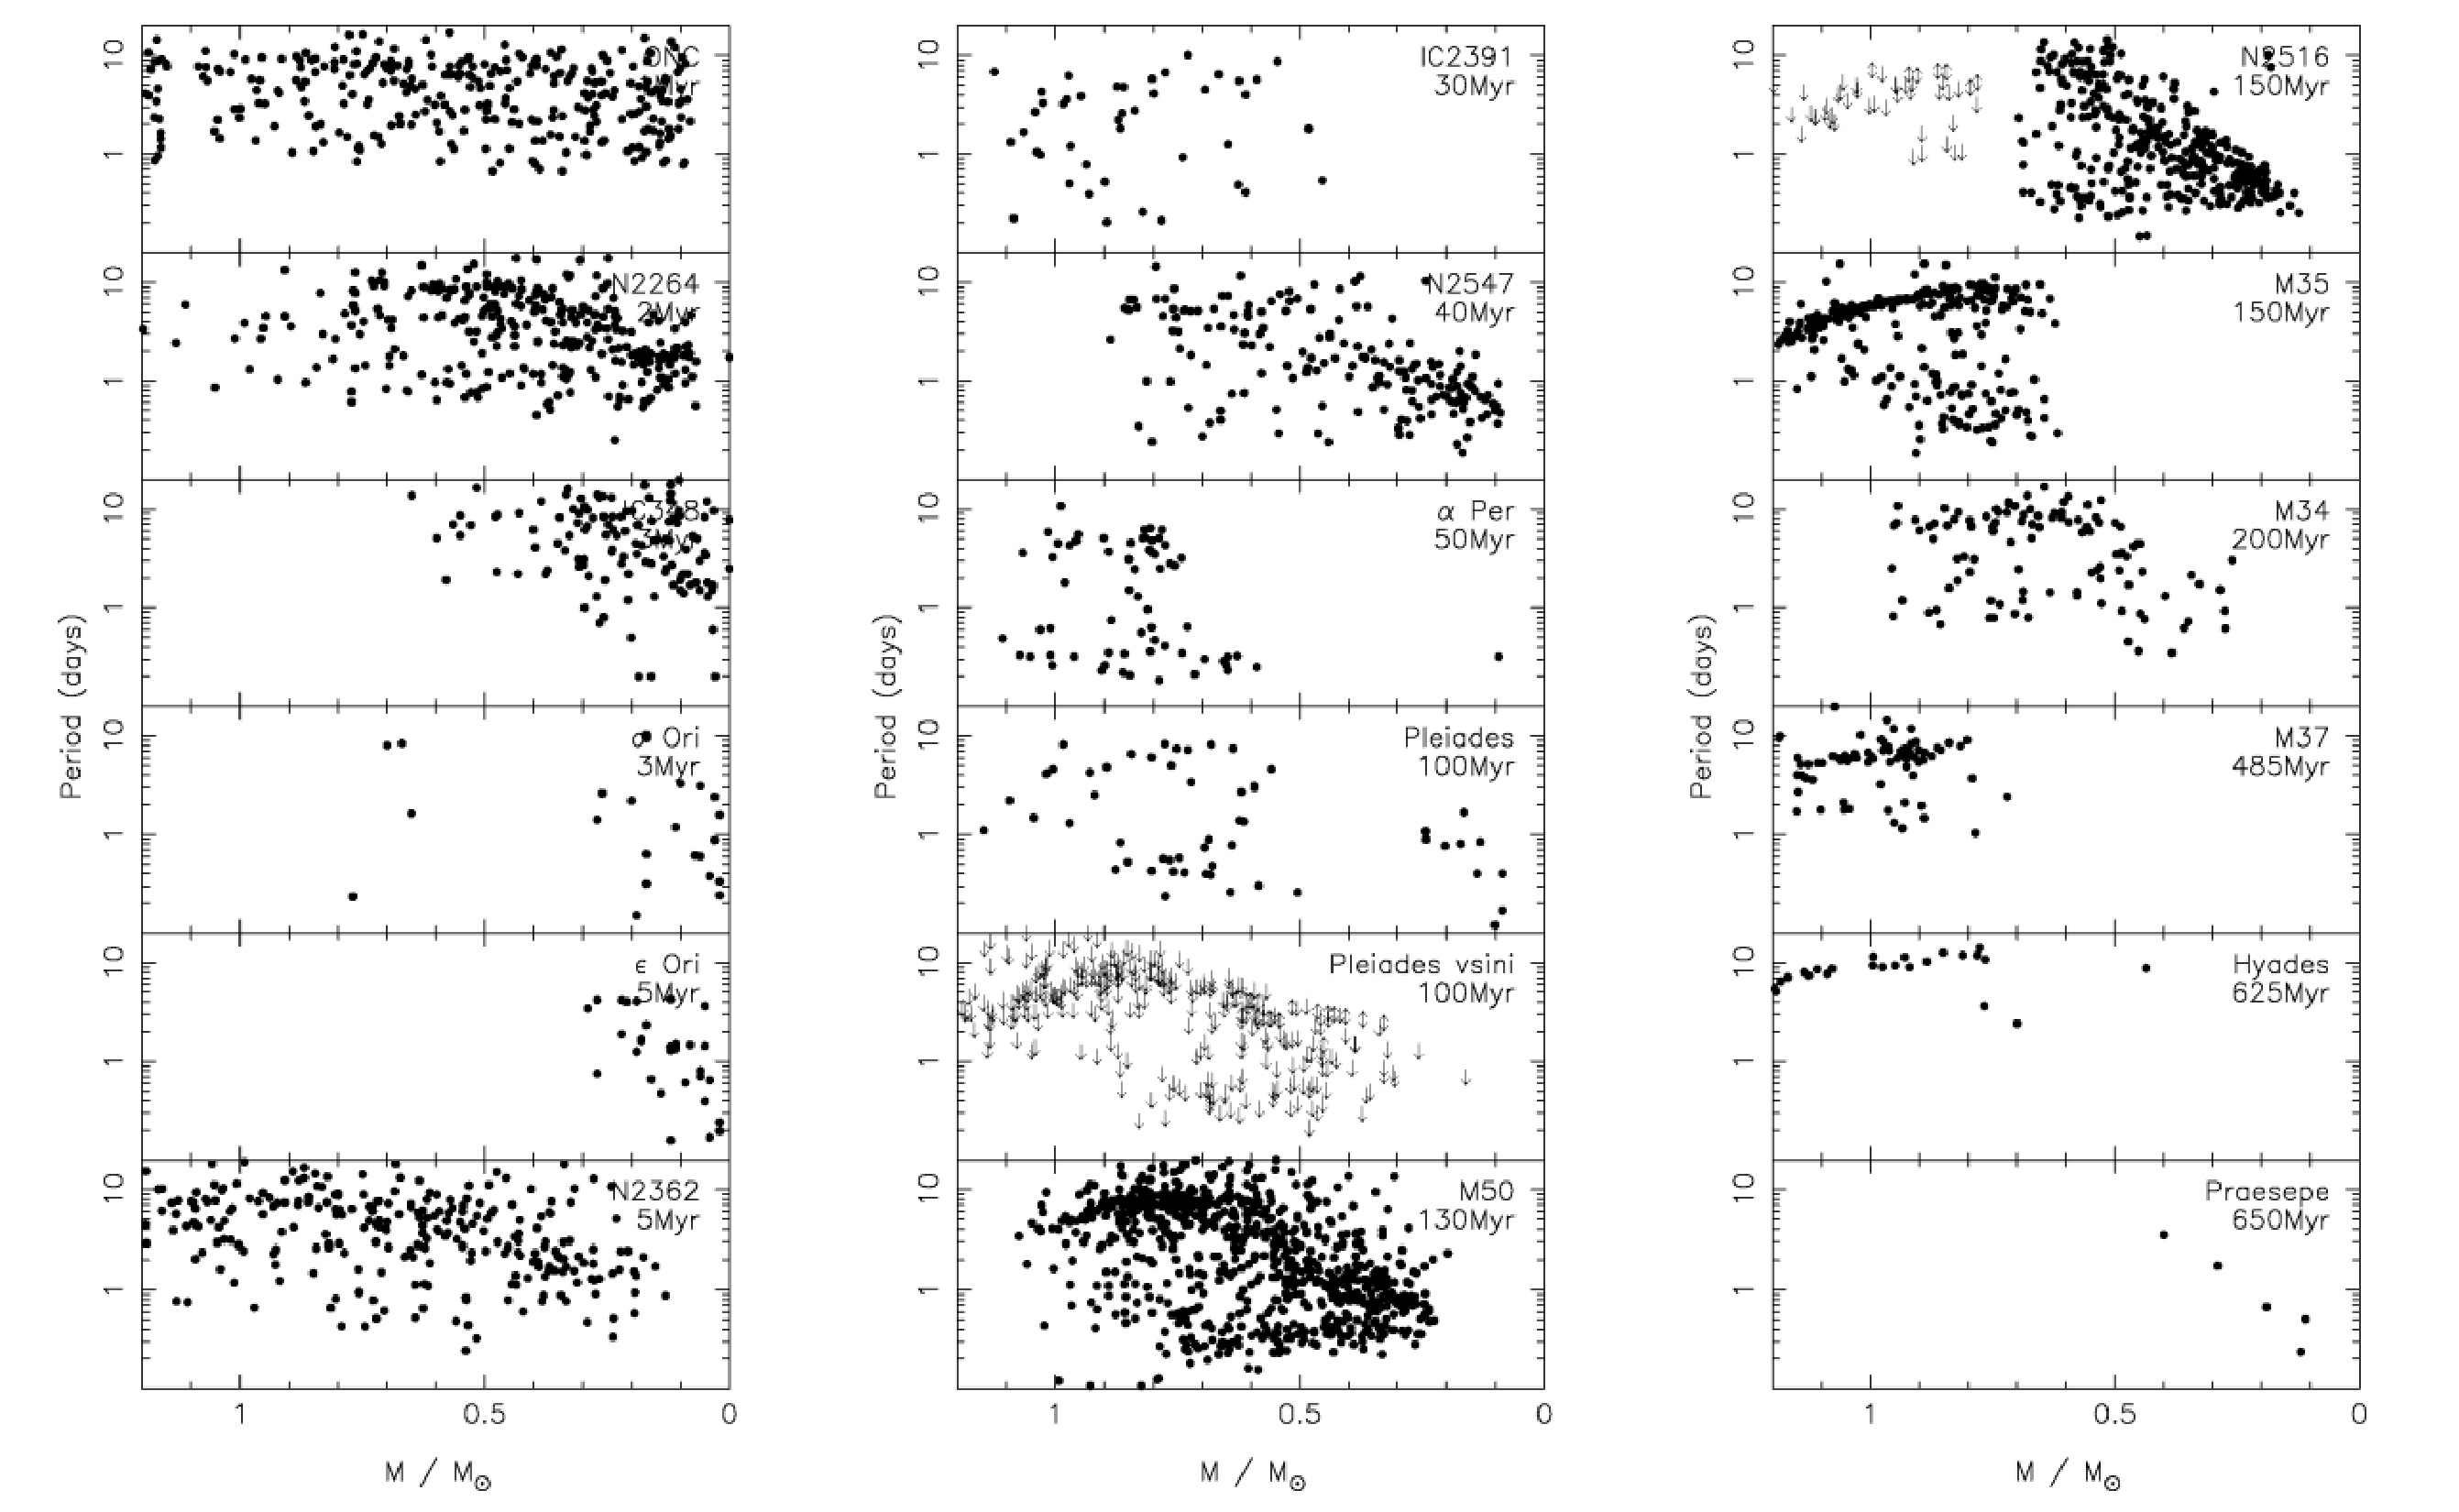
\includegraphics[width=6in, clip=true]{figures/irwin.pdf}
\caption[Cluster rotation from \citet{Irwin2009}]
{Figure from \citet{Irwin2009}. A compilation of most of the available
rotation periods for stars in open clusters with $M < 1.2 M_\odot$ in 2009.
Clusters increase in age from the top left to the bottom right.}
\label{fig:irwin}
\end{center}
\end{figure}


\citet{Barnes2003} pioneered an alternative approach to gyrochronology: an
entirely empirical one where simple functional forms are fit to the
observations \citep[\eg][]{Barnes2007, Mamajek2008}.
\citet{Barnes2003} proposed the following functional form for the relation
between period, colour and age,
\begin{equation}
P = A^n \times a(B-V-c)^b,
\end{equation}
\label{eq:Barnes2007_2}
where $P$ is rotation period (in days),
$A$ is age (in Myr), $B$ and $V$ are B and V band magnitudes respectively and
$a$, $b$, $c$ and $n$ are dimensionless free parameters.
\citet{Barnes2007} used rotation periods for stars in open clusters ranging in
age from 30-600 Myr to calibrate this relation.
% This same functional form was used by \citet{Mamajek2008} and who also used
% young clusters to recalibrate the gyrochronology model.

\citet{Barnes2010b} present a hybrid part theoretical, part empirical
gyrochronology relation:
\begin{equation}
\frac{dP}{dt} = \frac{\tau_c}{k_IP_{rot}},
\end{equation}
where $k_I$ is a dimensionless constant, calibrated with observations.
The convective overturn time, $\tau_c$ encodes the dependence on stellar mass.
In this thesis I use the \citet{Barnes2003} functional form because the only
available observables for the majority of \kepler\ stars are rotation period
and colour.
In the interest of using relatively model-independent parameters we avoid
calculating $\tau_c$.

\section{Other age diagnostics}
\label{sec:activity}

Isochrone fitting, asteroseismology and gyrochronology are probably the most
widely used dating methods today.
There are a handful of others available however, which I briefly outline
below.

\subsection{Magnetic activity}
% Rotation period decay is driven by the magnetic dynamo which also weakens over
% time.
% The slow decrease in magnetic field strength manifests in many ways.
Stars are born very active and become more inactive over time.
As well as decaying over billions of years, activity also varies on several
year timescales: the Sun, for example, has an 11 year activity cycle.
The activity cycle period, $P_{cyc}$ is related to rotation period, $P_{rot}$
via $P_{cyc} \approx (P_{rot}/\tau_c)^n$ where n $\approx$ 1.5
\citep{Noyes1984}.
Although stellar activity originates from one mechanism only, magnetism,
it manifests in a variety of detectable ways, listed below.
\begin{itemize}
\item{Star spots.
Surface differential rotation, where the equator rotates at a different speed
to the poles (in the Sun it rotates faster), twists magnetic flux into tubes
which emerge from the stellar surface.
The convection of material at the points where they emerge is inhibited and
these areas become cooler and darker as a result.
These cool, dark regions are called Sun spots on the Sun and star spots on the
surfaces of other stars.
Because these regions are darker, the integrated, optical flux emitted by a
star when there are more spots on the surface is decreased.
These decreases in brightness are detectable on the time scale of the stellar
rotation period, where spots rotate into and out of view, and on longer
timescales---the overall activity cycle.
% The Sun has an activity cycle that lasts 11 years.
% During periods of low activity the Solar surface has few star spots and this
% number increases up to hundred of spots during the Solar maximum.}
\item{Chromospheric activity.
Magnetic activity in stellar chromospheres produces emission in the cores of
singly ionised calcium H (3969.5$\AA$) and K (3933.7$\AA$) lines\footnote{The
H and K letters indicate the Fraunhofer designation.
Fraunhofer assigned letters to the absorption lines he detected in the Solar
spectrum.}.
This emission reversal is produced by the excitation of Ca$^+$ electrons to a
higher energy level via magnetic heating.
Just as with rotation period, chromospheric activity decreases with time and
the two properties are related \citep[\eg][]{Kraft1967, Noyes1984b}.
Relations between age and chromospheric activity have, just as with rotation
period, been calibrated \citep[\eg][]{Soderblom1991, Donahue1993,
Lachaume1999, Mamajek2008}.
Chromospheric activity is usually quantified via the R$\prime_{HK}$ index,
defined as the flux excess in the lines, normalised to the bolometric flux.
The limitations of using chromospheric activity indices as age diagnostics are
similar to the drawbacks of gyrochronology: the data are sparse and
particularly so at late ages and low masses.
Crucially though, measurements of Ca II H \& K emission are difficult to
obtain since high-resolution spectra are required ($R\gtrsim2000$).
}
\item{UV and X-ray flux.}
Magnetic heating in the chromosphere and corona excites photons to high
energies, producing substantial UV and X-ray fluxes
\citep[\eg][]{Pallavicini1981}.
Since M dwarfs have large convective zones, some even being fully convective,
they are highly active.
Their UV flux is significant and this topic is currently attracting attention
in the exoplanet community.
M dwarfs with transiting exoplanets are premium targets for follow-up with the
James Webb Space Telescope (JWST) since their petite size relative to their
Earth-radius planets provides deep transits.
The large S/N of these deep transits will allow JWST to search for biomarkers
in the atmospheres of these planets.
However, since M dwarfs are more active than G dwarfs, and their habitable
zones are closer in, any potential life on an Earth twin may have been
obliterated by the extreme UV flux.}
\item{Flare rate.
% Convective turbulence in low-mass stars generates magnetic flux tubes.
% Differential rotation then causes these flux tubes to twist around each other,
% becoming entangled.
Occasionally magnetic flux tubes reconnect, causing acceleration of particles
to enormous velocities, resulting in huge numbers of particles and amounts of
energy being released into the Inter-Stellar Medium (ISM).
These events are called flares.
The flare rate is related to the mean flare energy via a power law
\citep{Hawley2014, Davenport2015} and both of these properties are related to
the strength of the stellar magnetic field.
Flares occur extremely often in M dwarfs, the most magnetically active stars,
with energies ranging from $\sim e^{29} - e^{33}$ ergs and durations ranging
from a few to a hundred minutes \citep{Hawley2014}.}
% FIXME: what drives differential rotation?
\end{itemize}

\subsection{Lithium depletion boundary}
The Lithium Depletion Boundary (LDB) can be used as an age diagnostic for
young, low mass ($<1M_\odot$) stars.
As these young stars contract on the Pre-Main Sequence (PMS) their core
temperature increases.
When it reaches $\sim2.5\times10^6$ K, lithium is destroyed via $^7$Li$(p,
\alpha)^4$He and $^6$Li$(p, \alpha)^3$He proton capture reactions
\citep[\eg][]{Bodenheimer1965}.
The time taken for a star to reach these temperatures depends on its mass.
The lowest mass PMS stars are fully convective, so the mixing timescale is
very short and lithium depletion takes place very rapidly.
For young stellar groups therefore, the mass at which the LDB (the boundary
between stars that do and do not show lithium in their atmospheres) is located
is a very sensitive function of age \citep{Basri1996}.
LDB dating can be very precise but it is only applicable to young groups of
stars (20 Myr < age < 200 Myr) since by this time Lithium has disappeared from
the atmospheres of all members, regardless of their mass \citep{Burke2004}.

\subsection{Dynamics}
Stellar populations in the Milky Way galaxy can be localised into four groups:
the thin disc (containing the Sun), the thick disc, the bulge, and the halo.
Each of these stellar populations has a different distribution of stellar
ages.
The bulge is comprised of old stars and it is characteristically red because
the only remaining stars on the MS are low-mass.
The thin disc is comprised of young stars.
This is the main star-forming part of the galaxy as the spiral arms, density
waves of molecular gas that readily collapse into protostars, reside in the
thin disc.
The orbits of thin disc stars get heated over time.
Close encounters with neighbouring stars boost their orbital energies and many
thin disc stars find themselves `kicked' out of the galactic plane into the
`thick disc'.
The thick disc is statistically older than the thin disc since the majority of
its residents have had time to experience one or more close encounters.
The halo is even older still: these stars have been displaced even further
from the thin disc in which they were born.
Since the probability of experiencing a close encounter increases with time,
stars with higher proper motions are likely to be older \citep[see,
\eg][]{Shevelev1989, Nissen1991}.
However, although a rapidly moving star is likely to be older than a slowly
moving star, stellar-orbit heating is a stochastic process and therefore
cannot always be relied upon.

\section{Kepler}
\label{sec:kepler}

\begin{figure}[p]
\begin{center}
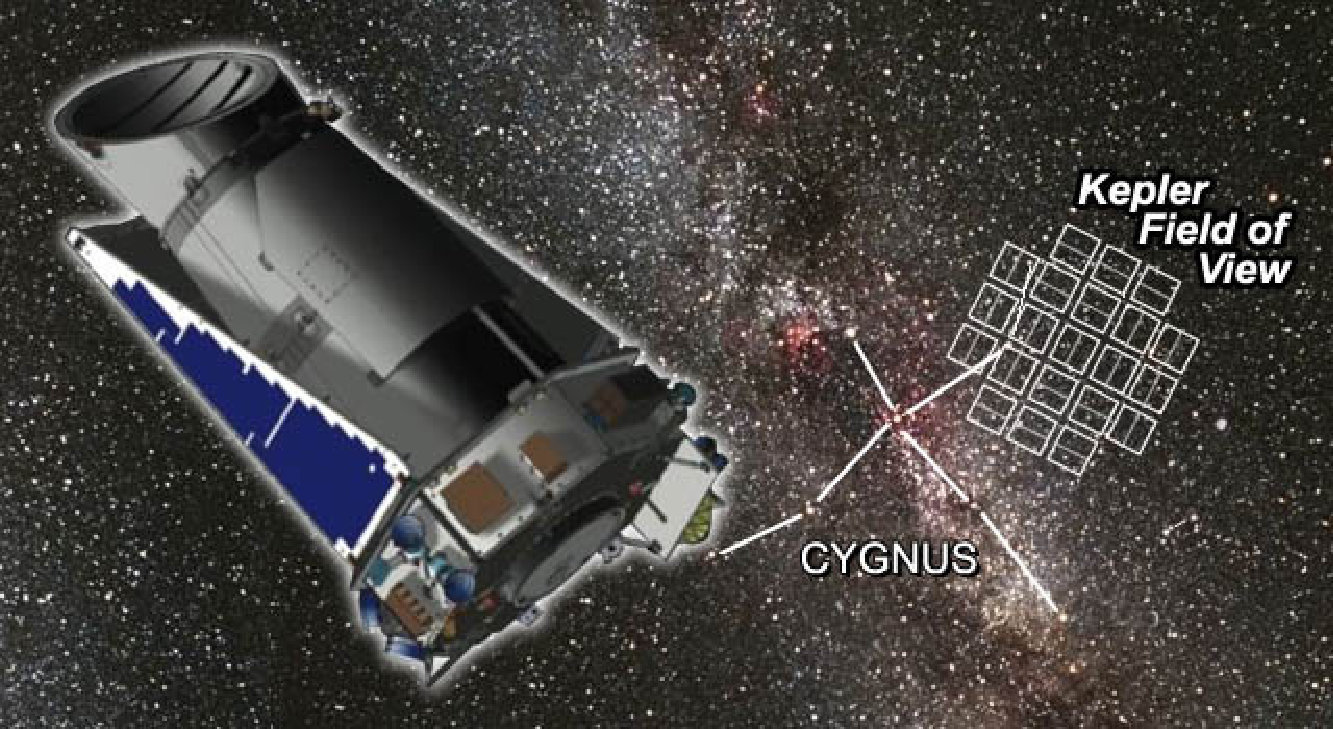
\includegraphics[width=6in, clip=true]{figures/kepler_pic.pdf}
\caption[The \kepler\ spacecraft and its field of view.]
{A depiction of the \kepler\ spacecraft and its field of view.
The \kepler\ field is located near the constellation Cygnus.
Image credit: \url{rst.gsfc.nasa.gov/Sect20/A11.html}}
\label{fig:current_fields}
\end{center}
\end{figure}

The \kepler\ spacecraft plays a starring role in this thesis.
\kepler\ was designed to survey over a hundred-thousand stars, searching for
extrasolar planets via the transit method.
Its ultimate goal was to answer the question "how common are Earth-like
planets in our galaxy?".
The first extra-solar planet orbiting a Sun-like star\footnote{The first
extra-solar planets were discovered orbiting a pulsar by observing pulsar
timing variations \citep{Wolszczan1992}.}
was discovered using the radial velocity method, whereby the presence of a
secondary body is inferred via the Doppler shift of the primary as it rotates
about the system's centre of mass \citep{Mayor1995}.
The first transiting exoplanet, HD 209458 b was discovered by
\citet{Charbonneau2000} using ground-based photometry.
Transits are produced when an exoplanet passes across the face of a star,
blocking a small section of the photosphere and producing a small dip in the
flux received at Earth.
In 2009, the \kepler\ telescope was launched --- a space mission dedicated to
searching for exoplanets via the transit method \citep{Borucki2010}.

The radial velocity and transit methods remain the dominant methods of
exoplanet detection.
Together, they produce an impressive catalogue of confirmed exoplanets.
Both methods, however, are subject to detection biases.
The depth of an exoplanet transit is proportional to the ratio of stellar and
planetary radii, squared.
The larger the planet relative to its host, the larger the dip and the easier
to detect.
In addition, planets with short orbital periods are also more easy to detect
due to the higher frequency of transit events.
This makes large planets orbiting small stars with short orbital periods the
easiest planets to detect.
Several studies have attempted to characterise the completeness and detection
efficiency of \kepler\ exoplanets in order to study their underlying
distribution \citep[\eg][]{Petigura2013, Foreman-Mackey2014,
Burke2015, Dressing2015}.
The radial velocity (RV) method is more sensitive to planets with a large mass
relative to their host star.
It is also easier to detect planets around old stars via the RV method since
magnetic activity can produce RV signals that can mask planet-induced Doppler
shifting \citep[\eg][]{Saar1997, Wright2005, Aigrain_2012, Rajpaul2015,
Rajpaul2016}.

An increasing number of planets have now been detected using direct imaging
\citep[\eg][]{Kalas2008, Nielsen2013}.
Using a coronagraph to block light from the host star and adaptive optical
instruments to cancel out disturbance from the atmosphere, it is possible to
observe emission from the surface of some planets at infrared wavelengths
where the planet is brightest.
It is only possible to directly image large exoplanets that are young and
still cooling from the formation process, therefore bright in infrared.
They should also have a large orbital separation from their host in order that
star light can be blocked without blocking radiation from the planet.
Direct imaging surveys are therefore currently limited in their detection
opportunities.
Yet another planet detection method is microlensing \citep[\eg][]{Abe2004,
Gould2010, Cassan2012, Gaudi2012}.
Occasionally, given near geometric alignment, light from a background (source)
star may be gravitationally lensed by a foreground star.
This process is detectable using time-series photometry if that foreground
star has high proper motion --- the source star appears to slowly brighten,
then fade over a matter of days as the lens passes in front of it.
If the foreground star has a planet it will produce an additional, lower
magnitude and much shorter increase in flux as it too passes in front of the
source.
Microlensing exoplanet surveys are again subject to different detection
biases than other methods.
To first order, detectability depends only on the mass ratio of planet and
star and the sky-projected separation between the two \citep{Clanton2016}.

Of all these methods, thanks to \kepler, the transiting method has been the
most fruitful to date.
\kepler\ has discovered more than 5700 planet candidates and over 1000
confirmed planets.
These numbers are still growing at a breath-taking rate and planets are likely
to continue being discovered in the data well after the \kepler\ funding has
dried up, thanks both to the enormity of the data set and the continual
improvement of planet search methods.
\kepler\ produced high precision\footnote{Precision ranging from a few hundred
parts per million for bright (< 13th magnitude) targets to tens of thousands
of ppm for faint (> 17th magnitude) targets.} broad-band (peaking between V
and R bands) light curves for $\sim$ 100,000 stars.
The majority of these targets were observed in long-cadence mode (once every
half-hour), and a few hundred in short cadence mode (once every minute),
continually for around four years.
% \kepler\ is in an Earth-trailing, heliocentric orbit.
The \kepler\ field is centred at $\mathrm{RA} = 19\mathrm{h}~22\mathrm{m}~
40\mathrm{s}$, $\mathrm{Dec} = +44^\circ30'~00'$, in the Cygnus region along
the Orion arm of the galaxy.
This field was chosen to be neither over nor under crowded, far enough out of
the ecliptic that the Sun never shines onto the detector and contamination
from Solar system objects is reduced.
\kepler\ has a limited amount of on-board storage and must point towards the
Earth to down-link data every month.
These pointings break the time series.
Other gaps appear at three month (quarter) intervals.
The spacecraft rotates every quarter to keep its Solar panels pointed at the
Sun.
The stars shift to new CCD modules every time this happens, eventually
returning to the same module after one year.
Both the down-link pointings and quarter rotations produce short gaps in the
light curves and can also produce short-term temperature changes to the CCD
which can effect the sensitivity of the detector.
Temperature changes increase the gain of the CCD chip: more electrons are
excited when the CCD is warmer so the flux appears to increase.
So despite the unprecedented precision of \kepler\ lightcurves, they are not
uninterrupted and contain systematic features.
A typical \kepler\ light curve is shown in figure
\ref{fig:demo_kepler_lightcurve}.
Understanding the systematics in \kepler\ data is necessary for {\it all} of
\kepler's science goals and is a key part of this thesis.
This point is covered further in \textsection \ref{sec:detrending}.

\begin{figure}[p]
\begin{center}
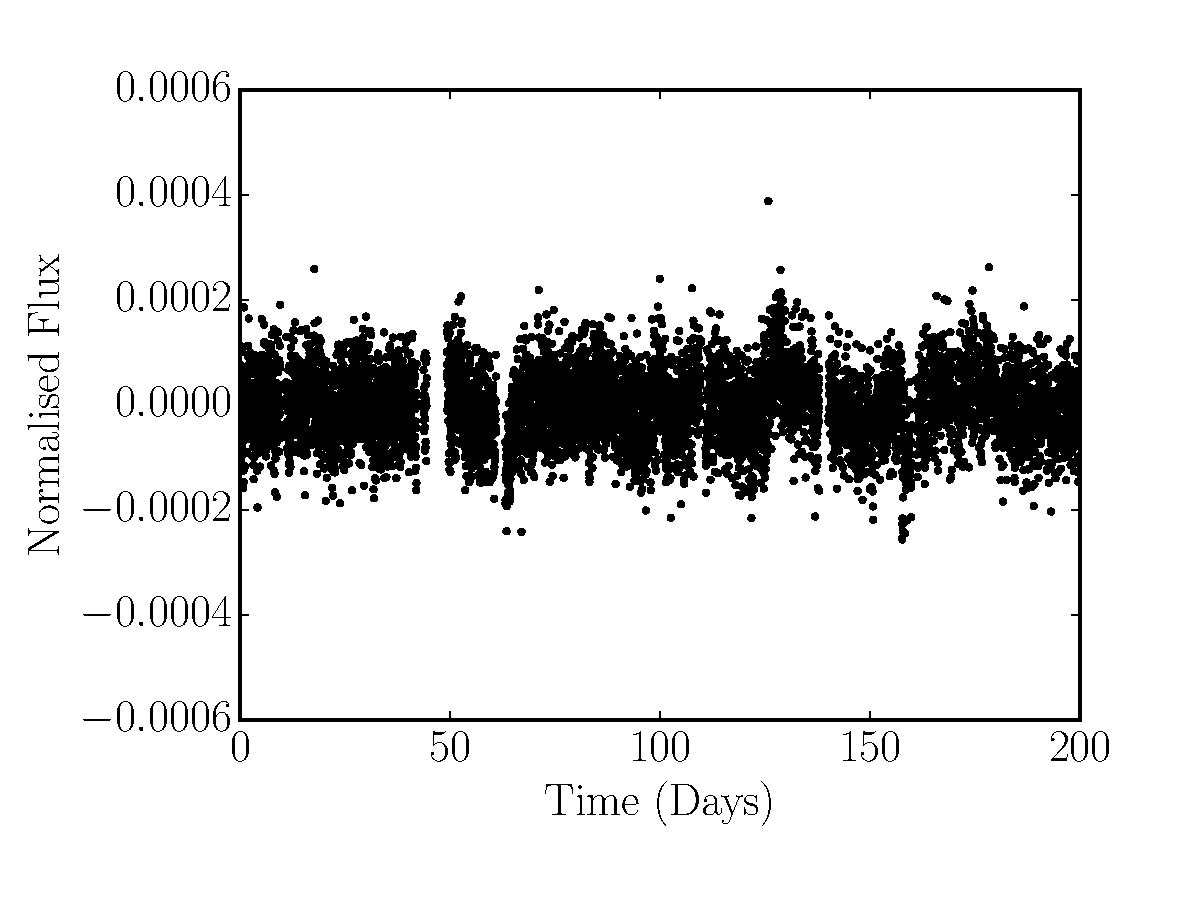
\includegraphics[width=6in, clip=true]{figures/demo_kepler_lightcurve.pdf}
\caption[An example \kepler\ light curve.]
{An example \kepler\ light curve.
In this figure, normalised flux versus time is shown for the first 200 days
of typical \kepler\ light curve, KID 2450729.
This is a relatively quiet star, although stellar variability is still present
at a low level.
Gaps in the data occur during quarterly spacecraft repointings and monthly
data downlinking.}
\label{fig:demo_kepler_lightcurve}
\end{center}
\end{figure}

Unfortunately, that key question---"how common are Earth-like planets?"---may
never be answered by \kepler\ \citep[or at least not very precisely. Several
inferences have been performed by extrapolation, \eg][]{Petigura2013,
Foreman-Mackey2014, Burke2015}.
Although \kepler\ launched with four functioning gyroscopic reaction wheels,
one broke shortly thereafter.
This was not a mission-ending scenario since the spacecraft only needed three
to maintain its precise pointing: one for pitch, one for roll and one for yaw.
Unfortunately however a second mission-critical reaction wheel
broke in 2013.
Without all three reaction wheels, precise pointing of the spacecraft was
impossible to maintain.
The extreme photometric precision of \kepler\ comes from its extreme pointing
position.
With stars fixed in place, moving by less than a few milli-arcseconds per
quarter, even without knowing the exact Point Spread Function (PSF) and Pixel
Response Function (PRF), it is possible to perform precise relative
photometry.
With its pointing stability compromised, the community were asked for input
for a repurposed \kepler\ mission \citep[\eg][]{Hogg2013, Aigrain2015}.

\kepler\ was re-purposed as the \ktwo\ mission in 2014.
With just two reaction wheels controlling pitch and yaw, its third rotation
axis had to be stabilised.
This was achieved by balancing the spacecraft against Solar pressure, using
its symmetric solar-panelled back.
The spacecraft sits in an unstable equilibrium, drifting slowly about its roll
axis, its new orientation reducing large forces from the Solar wind
\citep{Howell2014}.
The spacecraft's thrusters are used to correct the slow drift.
Although the precision is not what it once was, stars drift across several
pixels before the thrusters correct the motion, it is still good enough to
obtain huge amounts of useful data.
In order to keep its back to the Sun, \kepler\ can only point at fields in the
ecliptic plane.
This means that new stellar populations can be explored: from different
galactic regions, the bulge, thin and thick discs and halo, to open and
globular clusters.
Crucially, from the point of view of stellar astronomy, \kepler's new fields
incorporate several open clusters.
Open clusters are wonderful labs for stellar astronomy as they are coeval
populations of stars made from the same material.
They are controlled environments in which we can study the observational
properties of stars as a function of their mass.
Figure \ref{fig:current_fields} shows the current fields being observed by the
spacecraft and figure \ref{fig:future_fields} shows the future fields being
proposed.

\begin{figure}[p]
\begin{center}
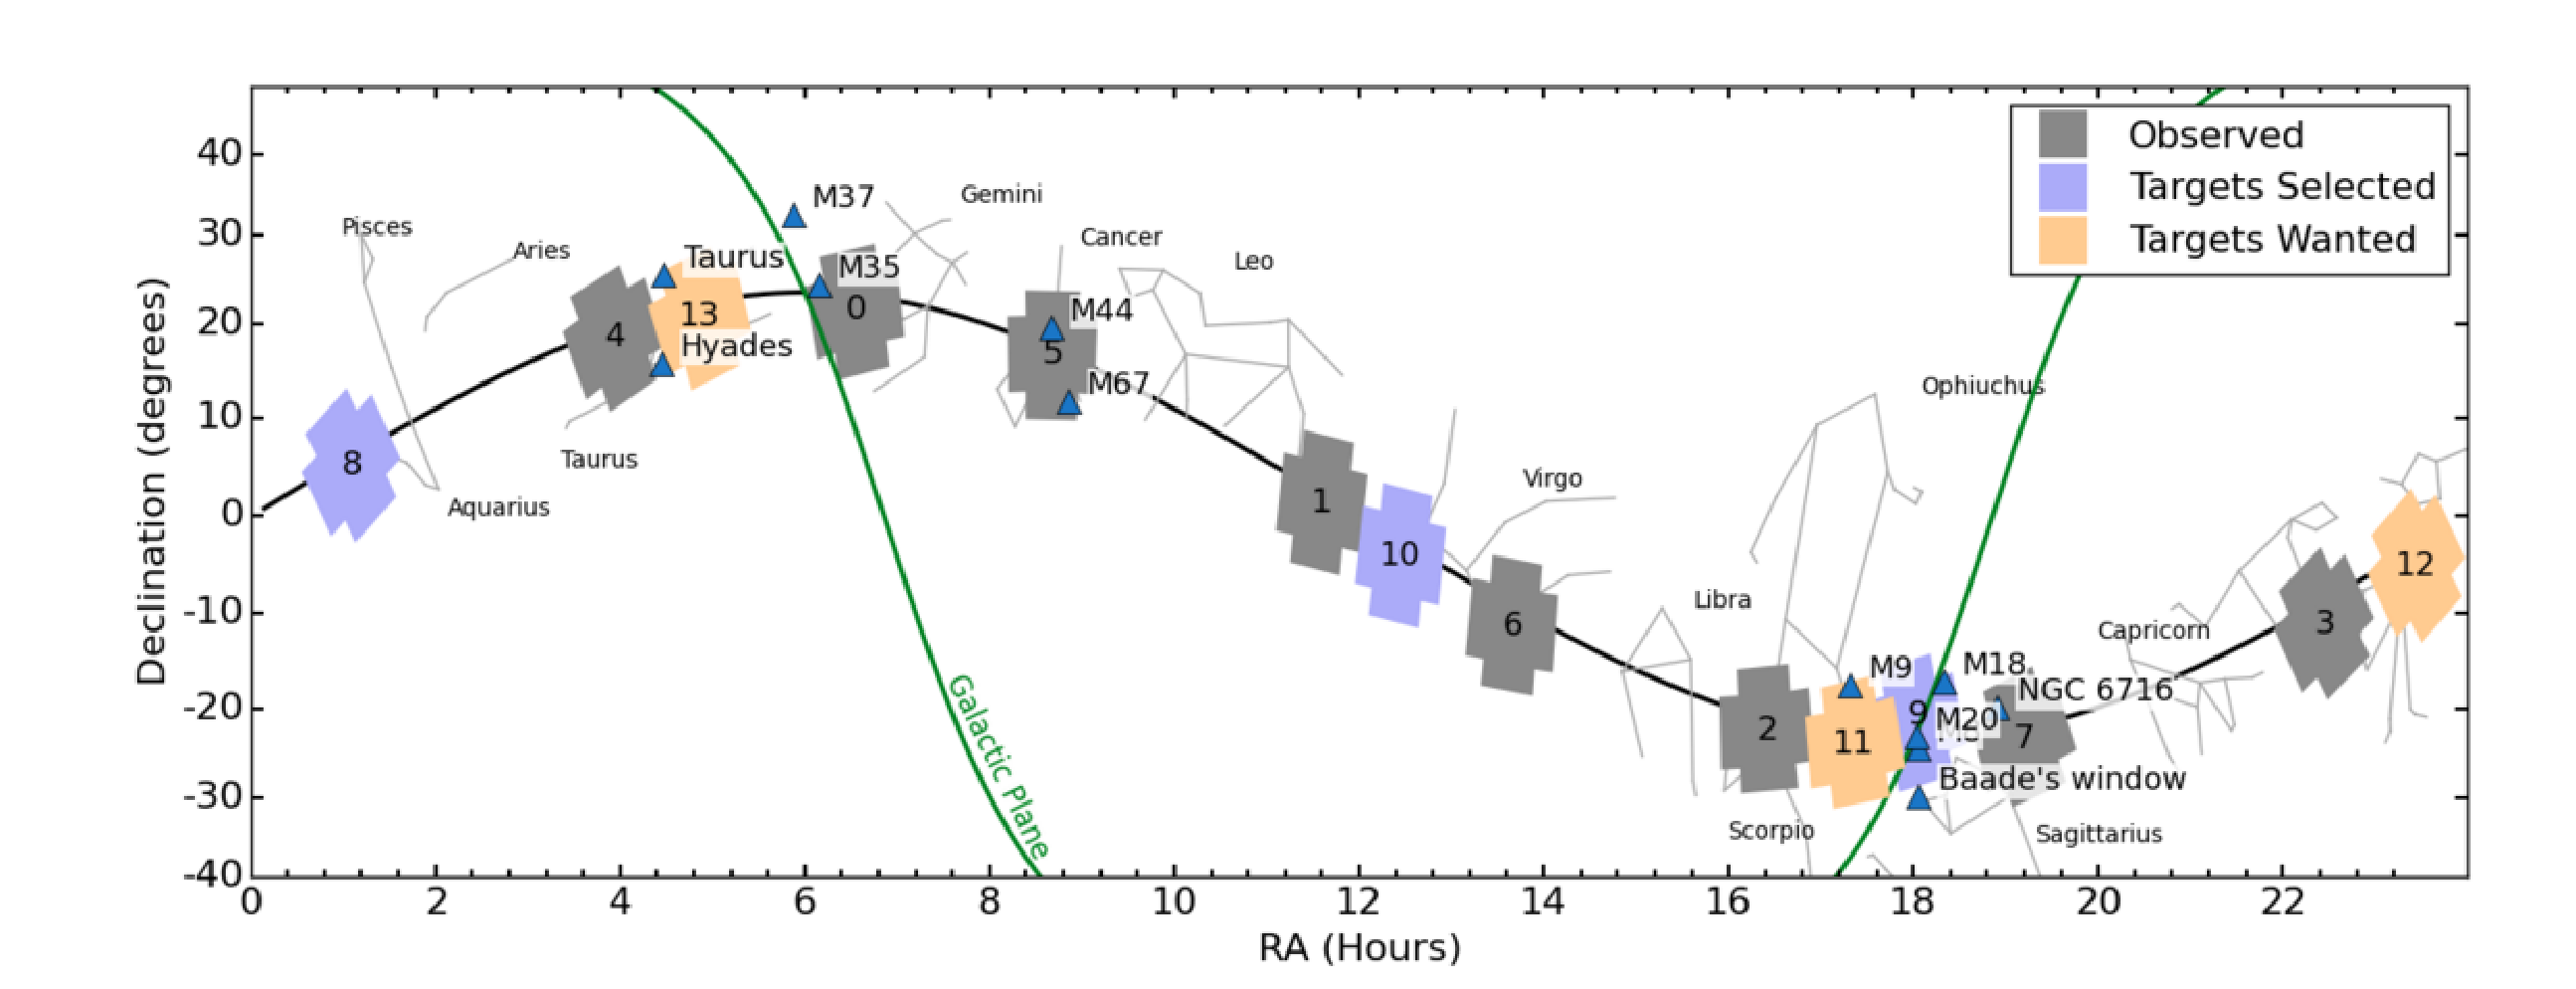
\includegraphics[width=6in, clip=true]{figures/Current_K2_fields.pdf}
\caption[Current \ktwo\ fields]{\ktwo's fields. Fields 1-9 have already been
observed and field 9 is being observed at the time this thesis is handed in.
Targets have been fixed for purple fields and proposals are currently being
solicited for yellow fields.}
\label{fig:current_fields}
\end{center}
\end{figure}

\begin{figure}[p]
\begin{center}
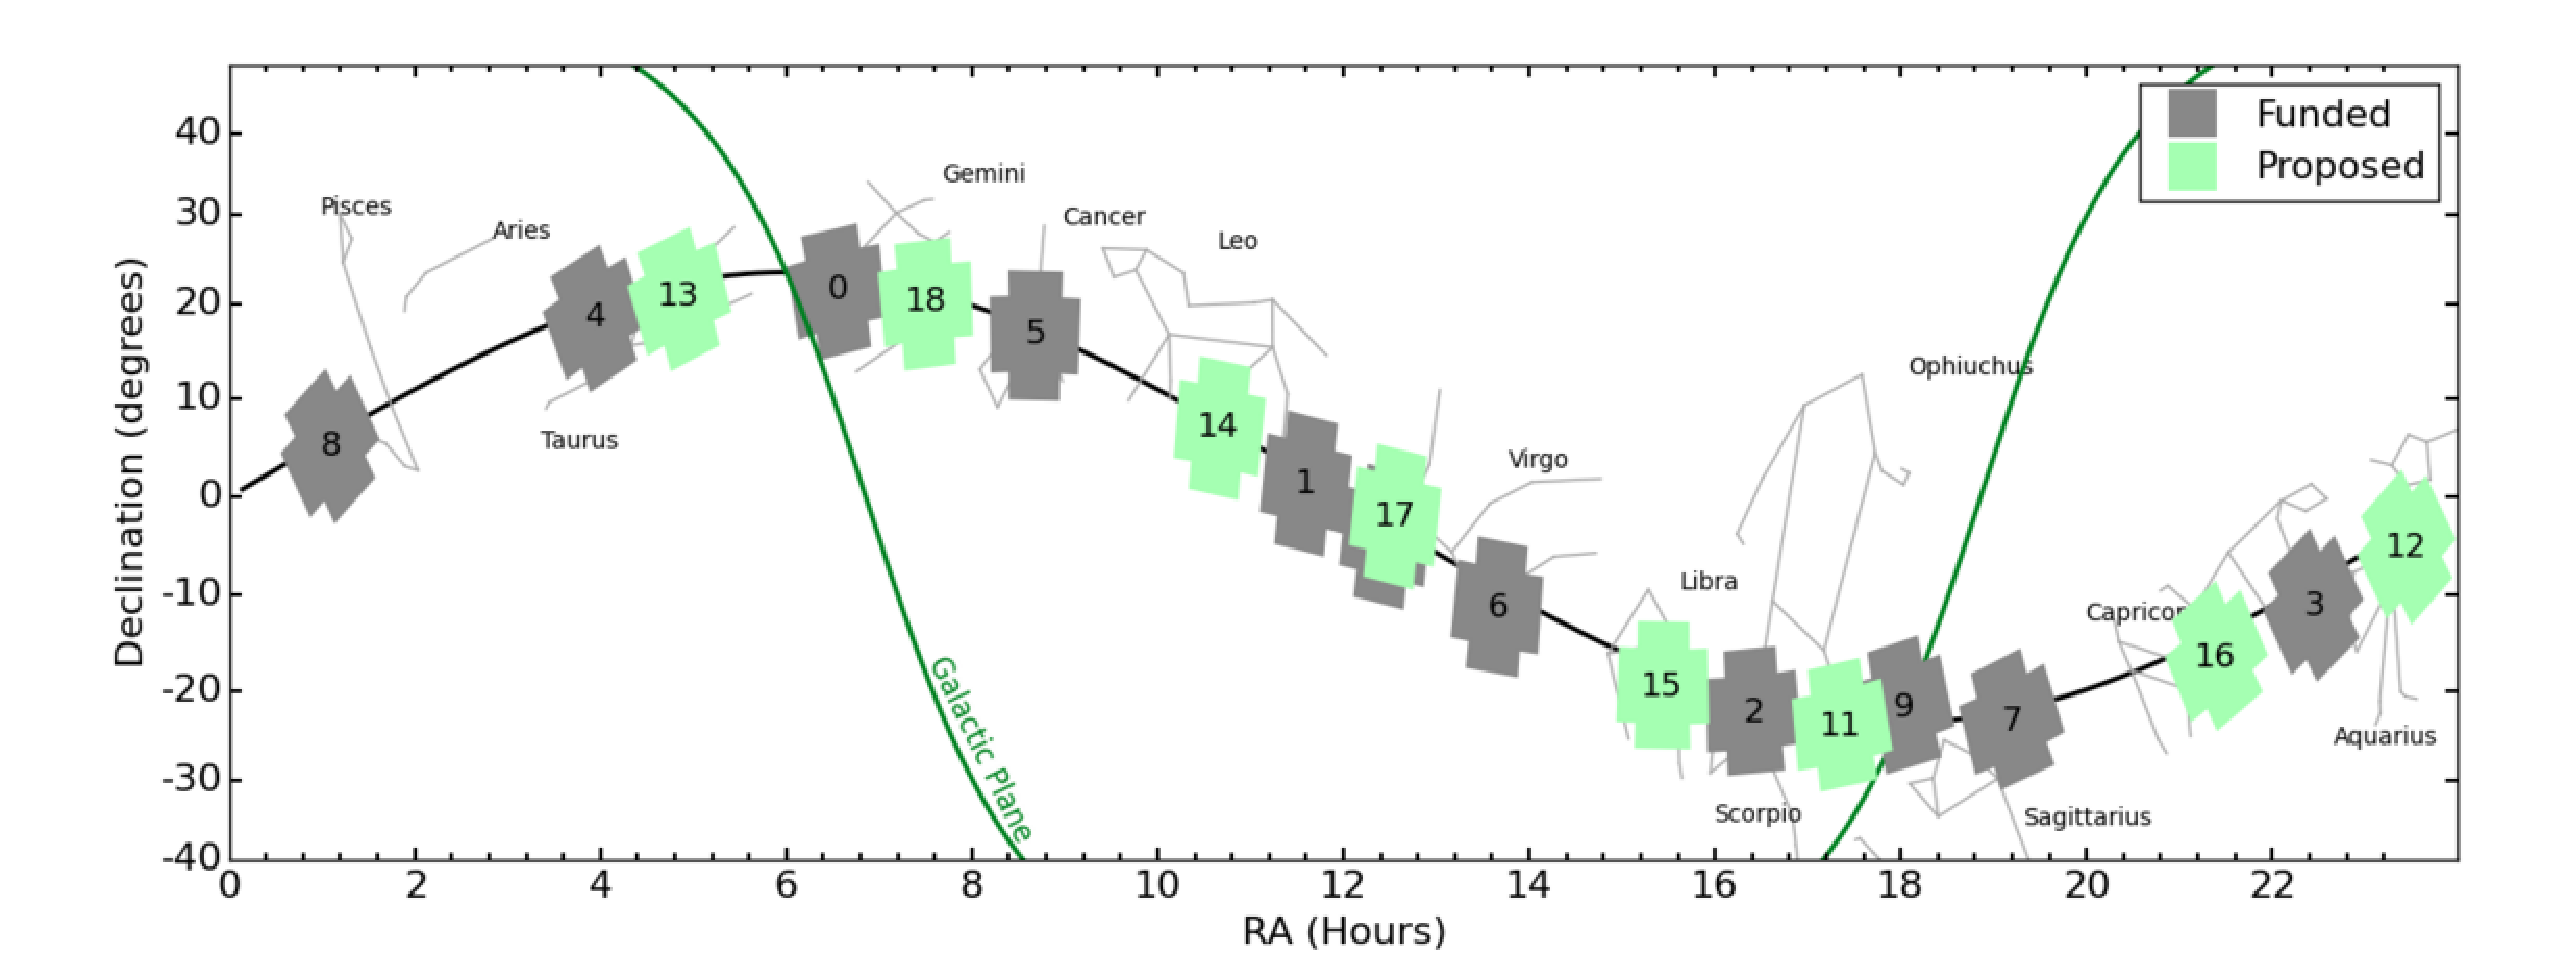
\includegraphics[width=6in, clip=true]{figures/Future_K2_fields.pdf}
\caption[Future \ktwo\ fields]{\ktwo's current and future fields. These green
fields are those proposed if an extended \ktwo\ mission is funded.}
\label{fig:future_fields}
\end{center}
\end{figure}

Not only is the spacecraft continuing its search for exoplanets \citep[and has
already discovered many, \eg][]{Vanderburg2015, Crossfield2015,
Foreman-Mackey2015, Montet2015, Becker2015, Vanderburg2016}, it will
provide time series of white dwarfs, active galactic nuclei, red giants, red
dwarfs, binary stars and other interesting astronomical objects.
Of course, with the reduced pointing position comes a new challenge for those
astronomers willing to get their hands dirty: systematic features in \ktwo\
light curves range from negligable for the brightest targets to overwhelming
for the faintest.
It is therefore necessary to employ heavy-duty `detrending' methods to
exploit \ktwo's rich data set.
This subject is covered in \textsection \ref{sec:detrending}

\section{Statistical methods}

A theme continued throughout this thesis is probabilistic statistical methods.
None of the methods used here are new in themselves, but many have not been
previously used on the sorts of problems presented here, or in an astronomical
context.
% I will now discuss them in the order in which they feature in the subsequent
% chapters of this thesis.

\subsection{Multi-dimensional and unknown uncertainties: hierarchical
probabilistic modelling}
In some astronomical data sets, only the dependent variable has significant
uncertainties---for example in time-series or spectra---in which case it is
reasonable to ignore independent variable uncertainties.
When performing regression on data with only $y$-direction, Gaussian
uncertainties where the measurements are independent and there is no
correlated noise, it may be appropriate to use a simple Gaussian likelihood
function.
For example, the likelihood of $y$-values given some $x$-values, some model
parameters, $\mathbf{\theta}$ and some $y$-direction uncertainties, $\sigma$,
can be written
\begin{equation}
    p(\{y\}_{i=1}^N|\{x\}_{i=1}^N, \{\sigma\}_{i=1}^N, \mathbf{\theta})
    = \prod_{i=1}^N \frac{1}{\sqrt{2\pi\sigma_i^2}}
    \exp\left(-\frac{[y_i - \mu(x_i, \mathbf{\theta})]^2}{2\sigma_i^2}\right),
\end{equation}
where $\mu$ is the mean model.
It is often more practical to use the logarithm of this function,
\begin{equation}
    \ln\mathcal{L} =
    -\frac{1}{2} \sum_{i=1}^N \left[\frac{[y_i - \mu(x_i,
    \mathbf{\theta})]^2}{\sigma_i^2} +
    \ln\left(2\pi\sigma_i^2\right) \right].
\end{equation}
\label{eq:lnlike_intro}

In many fitting-a-model-to-data problems in the astronomical literature, a
frequentist approach is taken and $\chi^2$ is minimised (or log-likelihood is
maximised).
The probabilistic (Bayesian) approach however, is to multiply this likelihood
by a prior to produce a posterior Probability Density Function (PDF):
\begin{equation}
    p(\theta|\{y\}_{i=1}^N, I) = \frac{p(\{y\}_{i=1}^N|\theta, I)
    p(\theta, I)}{p(\{y\}_{i=1}^N|I)}.
\end{equation}
In this equation, $I$ is used to represent all of one's knowledge and
implicit assumptions made about the data and the model.
The prior, $p(\theta, I)$ represents one's prior beliefs about the model
parameters, $\mathbf{\theta}$.
There is a wide range of literature available on the science behind choosing
priors which is beyond the scope of this thesis \citep[\eg][]{Kass1996,
Gelman2009, Vanderplas2014}.
The denominator in the above equation is the likelihood of the data,
marginalised over all model parameters.
Is is sometimes known as the `fully marginalised likelihood' and sometimes the
`evidence'.
It is a useful quantity to compute when performing model comparison but not
is necessary for performing regression.
I do not perform model comparison here so a discussion of the evidence
integral is beyond the scope of this thesis.

Returning to the equation for the log-likelihood, equation
\ref{eq:lnlike_intro}, it is trivial to modify this function for the case
where the $y$-direction uncertainties are unknown, under, or over-estimated.
In this case one could write
\begin{equation}
    \ln\mathcal{L} =
    -\frac{1}{2} \sum_{i=1}^N \left[\frac{[y_i - \mu(x_i,
    \mathbf{\theta})]^2}{\sigma_i^2 + s^2} +
    \ln\left(2\pi(\sigma_i^2 + s^2\right) \right],
\end{equation}
where $s^2$ is the additional variance needed to explain the scatter in the
data.

In chapter \ref{chapter:flicker} a modification to the above equation is used
to fit a line to data where the uncertainties are underestimated.
This is a hierarchical problem since there are two parameters that describe
the model (a straight line), $\alpha$ and $\beta$, where $\mu = \alpha +
\beta x$ and a parameter describes the standard deviation of a Gaussian
spanning the mean model.
In other words, the `true' value of variable $y$---the value that would have
been measured if there were no observational uncertainties---
$\bar{y}$, is drawn from a Gaussian with mean, $\mu = \alpha + \beta \bar{x}$
and standard deviation, $s$:
\begin{equation}
\bar{y} \sim \mathcal{N}(\alpha + \beta\bar{x}, s^2),
\end{equation}
and the {\it observations}, $y_{obs}$ are in turn drawn from Gaussians with
$\mu = \bar{y}$ and standard deviations described by the individual
observational uncertainties, $\sigma_{obs}$:
\begin{equation}
y_{obs} \sim \mathcal{N}(\bar{y}, \sigma_{obs}^2).
\end{equation}
Since it is the observations that are modelled, not the latent parameter,
$\bar{y}$, this is a hierarchical process.

Equation \ref{eq:lnlike_intro} can also be modified for the simple case of
fitting a straight line to data, where the $y$-direction observational
uncertainties are unknown {\it and} the $x$-direction uncertainties are
non-negligible.
Starting from equations 26, 29, 31 and 32 of \citet{Hogg2010b},
$\mathbf{S_i}$ is the covariance tensor,
\begin{eqnarray}
    \mathbf{S_i} &\equiv& \left( \begin{array}{cc}
                    \sigma_{x}^2 & \sigma_{x,y} \\
                    \sigma_{x,y} & \sigma_{y}^2
\end{array}\right),
\end{eqnarray}
\label{eq:covariance_tensor}
$\mathbf{\hat{\nu}}$ is a unit vector orthogonal to the line with slope
$\alpha$,
\begin{equation}
    \mathbf{\hat{\nu}} = \frac{1}{\sqrt{1 + \alpha^2}} \left( \begin{array}{c}
                                                    -\alpha \\
                                                    1
    \end{array}\right),
\end{equation}
\label{eq:unit_vector}
the variance of the data is given by,
\begin{equation}
    \Sigma_i^2 = \mathbf{\hat{\nu}}^T \mathbf{S_i} \mathbf{\hat{\nu}}
\end{equation}
\label{eq:variance}
and the log-likelihood is,
\begin{equation}
    \ln\mathcal{L} = - \frac{1}{2} \sum_{i=1}^N \left[
    \frac{\Delta_i^2}{\Sigma_i^2} + \ln|\mathbf{S_i}| \right].
\end{equation}
\label{eq:ndlnlike}
By modifying equation \ref{eq:covariance_tensor} to be
\begin{eqnarray}
    \mathbf{S_i} &=& \left( \begin{array}{cc}
                    \sigma_{x}^2 & 0 \\
                    0 & \sigma_{y}^2 + s^2
\end{array}\right),
\end{eqnarray}
\label{eq:covariance_tensor_mod}
since we assume that the covariance between $x$ and $y$ is negligible,
substituting \ref{eq:covariance_tensor_mod}, \ref{eq:unit_vector} \&
\ref{eq:variance} into \ref{eq:ndlnlike} gives
\begin{equation}
    \ln(\mathcal{L}) = -\frac{1}{2} \sum_{i=1}^N
    \left( \frac{\left[ y_i - (\alpha + \beta x_i) \right]^2}
    {\beta^2\sigma_{x, i} + \sigma_{y, i}^2 + s^2} + \ln[\sigma_{x,
    i}^2(\sigma_{y, i}^2 + s^2)]
    \right).
\end{equation}
This is the equation used in chapter \ref{chapter:flicker} to analyse
astrophysical data with intrinsic scatter.

In cases with more complicated mean models, it is not so easy to arrive at an
analytic solution.
For example, a similar problem is approached in chapter \ref{chapter:gyro}.
Here, the extra variance parameter, $s$, is not used (although it should be
included in future analyses!), however the uncertainties in the $x$, $y$, and
this time $z$, directions are large.
The model is not a simple two-dimensional line as in the above case, it is the
three-dimensional gyrochronology equation \ref{eq:Barnes2007_2} where $y$ is
rotation period, $x$ is age and $z$ is B-V colour.
In this case, an approximation must be made in order to take the uncertainties
on all dimensions into account.
This approximation is made via sampling and is described in chapter
\ref{chapter:gyro}.

\subsection{Methods for removing systematics}
\label{sec:detrending}

`Detrending' is a word that has been adopted by astronomers to mean removing
systematic trends caused by non-physical (\ie\ instrumental) variations in the
experiment conditions.
This process can be applied to any data set that contains correlated noise, be
it a time series, image or spectrum.
However `detrending' usually pertains specifically to time series analysis,
and light curves in particular.
The detrending process involves generating some model of the systematic
features which is then subtracted from the light curve.
This implies that the contribution of systematics to the light curve are known
{\it a priori}.
Of course in reality, the contributions coming from the signal and the noise
can never be separated completely, so this is an approximate process.
In some cases this approximation is close to the truth, or close enough---for
example, if signal and noise look very different, rough detrending may still
reveal useful signals in the data.
However, in many cases the noise model cannot be adequately approximated.
At best this leads to inaccurate inferences about the physical system being
studied and at worse it leads to false positive detections and false negative
non-detections.

In \textsection \ref{chapter:sip} I present a method for extracting periodic
signals from \ktwo\ light curves, without detrending.
Here I summarise the detrending process for the original \kepler\ mission.

\kepler\ data is available to download at various stages of the reduction
process.
Target Pixel Files (TPFs), are arrays of the raw pixel fluxes, Simple Aperture
Photometry (SAP) light curves are generated by combining pixel fluxes with
simple masks and Presearch Data Conditioned, Maximum {\it A Posteriori}
(PDC-MAP) light curves, are a detrended data product.

The detrending process concerns removing as much of the noise as possible
whilst preserving the signal \citep{Smith2012, Stumpe2012}.
In reality no detrending process does this perfectly and most favour a
slightly more or less aggressive approach to removing systematics, depending
on the science goal.
Systematic features in \kepler\ light curves are generated by two main
sources: pointing variations and temperature variations (although pointing
variations are more serious for \ktwo\ light curves than \kepler\ light
curves).
Regardless of the source, either of these variations will effect stars that
lie close together on the CCD in similar ways.
The \kepler\ pipeline uses this fact to isolate physical signals from
instrumental: physical signals vary from star to star and instrumental signals
are present in nearby groups of light curves.
Intrinsically quiet stars that are nearby, but display similar patterns in
variation, are used to generate a set of Cotrending Basis Vectors (CBVs) via
Single Value Decomposition (SVD).
A detrending model, constructed from a linear combination of CBVs is then fit
to these stars and the distribution of the CBV weights are used to generate a
prior.
A systematics model is then fit to each individual light curve, where a
likelihood function is multiplied by the prior and the resulting maximum of
the posterior PDF is taken to be the best fit.
That systematics model is then subtracted from the data.

PDC-MAP light curves were designed to maximise exoplanet transit search
capability.
These signals are rarely longer than thirteen hours and have a characteristic
upside-down top-hat shape.
Stellar variability on the other hand is smoothly varying (similarly to
systematic features) with timescales ranging from around one day to several
years.
PDC-MAP detrending does not preserve signals longer than $\sim$ 30 days.
% FIXME: find this CITATION

An alternative approach to PDC-MAP detrending, designed to preserve signals
from the stars as {\it well} as the planets is that of \citet{Roberts2013}.
They also fit a linear combination of CBVs to the data, however the main
differences in their approach are to impose a maximum entropy criterion:
trends in the most highly-weighted CBVs must be present in a large number of
light curves, and to remove high frequency noise from the systematics model
before detrending so as not to inject high frequency noise.
A comparison of the two detrending methods is presented in
\citet{Roberts2013}.

Once \kepler\ lost its third reaction wheel, pointing variations became much
more severe, systematic features rose in amplitude and more aggressive
detrending techniques became necessary.
In chapter \ref{chapter:sip}, I introduce an alternative to detrending,
specifically applicable to \ktwo\ light curves.

\subsection{Rotation period inference}
\label{sec:rotation}
The overall brightness of stars is periodically reduced by spots on their
surfaces.
A measurement of the time between successive dimmings provides an indication
of the surface rotation period.
Unfortunately, inferring accurate rotation periods is not as simple as finding
the period of the best-fit sinusoid: the picture is complicated by several
factors:
\begin{itemize}
\item{The presence of {\it several} dark spots and plages (bright spots), with
complicated geometries, on the surface at any given time creates
non-sinusoidal brightness variations.}
\item{Spots are born, grow, then shrink and eventually fade away.
The finite lifetimes of spots produces evolving patterns in light curves.
Furthermore, spots are born at a range of longitudes, meaning that brightness
variations are not perfectly periodic.}
\item{Many stars exhibit signs of differential rotation, \ie\ the poles and
the equator rotate at different angular velocities.
Star spots may be present at multiple latitudes simultaneously which will blur
the periodicity of the signal---it will have a finite width in frequency
space, rather than appearing as a delta function.
If there are two dominant active regions at different latitudes, two distinct
periodic signals may be present in the light curve.
The famous butterfly diagram for the Sun demonstrates that solar spots are
born at active latitudes, bands around 30$^\circ$ in width, between 0 and
30$^\circ$ north and south of the equator \citep[\eg][]{Charbonneau2010}.
Spots are born at lower and lower latitudes over the course of one Solar
cycle, therefore if the Sun were a \kepler\
star one would measure a different rotation period from one year to the next.
}
\end{itemize}

In this thesis I will take `rotation period' to mean the equatorial period.
For stars with significant differential rotation, this will be the minimum
rotation period (assuming that equatorial rotation is faster than polar
rotation, as in the Sun).
In reality therefore, all photometric rotation periods are just upper limits.
This is an interesting point for a future discussion but is beyond the scope
of this thesis.

\citet{Aigrain2012} and \citet{Dumusque2014} demonstrate the effects of spots
on the flux variations of stars and provide realistic models for translating
flux signals into Radial Velocity (RV) signals\footnote{There is now a large
body of (occasionally controversial) literature on this topic in the context
of exoplanet search.
Star spots signals can look like exoplanet signals in RV time series.
Modelling star spots has now become a necessity for exoplanet RV search.}.
These models include parameters such as period, inclination, number of spots,
spot lifetime, spot temperature, differential rotation amplitude (shear), and
others.
They are able to produce light curves that look very similar to real \kepler\
time-series, however fitting such models to data is not straightforward.
It is impractical to have a set of parameters (\eg\ latitude, longitude, size,
temperature) for each spot, however it is difficult to simplify the model in a
way that will allow enough flexibility to fit a real data set.
It is therefore necessary to use alternative methods for inferring rotation
periods.
In chapter \ref{chapter:GP} of this thesis I present a new method for
inferring rotation periods, and give a summary of the main existing methods
below.

\subsubsection{Lomb-Scargle periodograms}
Lomb-Scargle (LS) periodograms \citep{Lomb1976, Scargle1982} were developed
by astronomers to perform frequency analysis on unevenly spaced data.
To produce a LS periodogram, a sinusoid is fit to a time series via
least-squares over a grid of frequencies.
The amplitudes of the sinusoid are plotted against frequency to produce a
power spectrum.
This is simple linear regression and LS periodograms are therefore
inexpensive to compute, although more costly than Fast Fourier Transforms
(FFTs).
% QUESTION: learn FFT operations.
LS periodograms have been used to study periodic phenomena in astrophysical
time series for decades and were the first tools used to measure photometric
rotation periods \citep[\eg][]{Scott1992, Mottola1995}.
They are often use to infer rotation periods from \kepler\ light curves
\citep[\eg][]{Reinhold2013, Reinhold2013b}.
The main drawback of the LS periodogram for rotation period measurement is
that a sinusoid is not necessarily a good model for the kinds of signals
produced by star spots and results in imprecise period measurement.
This is not a problem however, for the ACF method.

\subsubsection{The ACF method}

An AutoCorrelation Function (ACF) is often used to measure stellar rotation
periods \citep[\eg][]{Aigrain2008, Mcquillan2013, Mcquillan13b,
Mcquillan2014, Garcia2014}.
A method was developed specifically for \kepler\ data by
\citet{Mcquillan2013}.
The ACF itself is defined as
\begin{equation}
    r_k = \frac{\sum_{i=1}^{N}(x_i-\bar{x})(x_{i+k}-\bar{x})}
    {\sum_{i=1}^{N}(x_i-\bar{x})^2},
\end{equation}
where $r_k$ is the autocorrelation coefficient at lag $k$ for a time series
with elements, $x_i~(i=1,..., N)$.
An ACF is only applicable to time series with evenly spaced data (which is
usually an acceptable approximation for \kepler\ light curves) and a Fourier
transform of an ACF is the power spectral density.

Unlike the LS periodogram which uses a sinusoid to fit the data, because the
ACF does not rely on a functional form---it simply looks for repeating
patterns---it is better suited to measuring stellar rotation periods,
particularly for relatively inactive stars where long time series are required
to detect the weak rotational signal \citep[see][for an in-depth
discussion]{Mcquillan2014}.
A series of uniformly spaced peaks will be visible in the ACF of a light curve
with a rotational signal.
The position of the first peak corresponds to the lag-time of greatest
correlation.
This peak is usually adopted as the rotation period.
However, if the second peak is higher than the first, {\it that} will be taken
as the rotation period.
This is usually caused when there are two active regions on opposite
hemispheres of the star, $\sim$ 180$^\circ$ apart, producing two dips in the
light curve per rotation period.
The ACF method was used by \citet{Mcquillan2014} to measure rotation periods
of 34,030 \kepler\ targets.

The main drawback of the ACF method is that uncertainties are not well
defined.
ACF rotation periods with uncertainties reported in the literature are
typically measured by fitting a Gaussian to the peaks in the ACF.
However, the width of the ACF peak is related to the rate of correlation
coefficient fall-off which depends on the shape of the signal and cannot be
interpreted as a measurement uncertainty, $\sigma$.
Although the ACF method is better suited to rotation period signals than the
LS periodogram, it is not suited to model quasi-periodic signals which will
act to broaden peaks in the ACF.

\subsubsection{Wavelets}
Wavelet transforms are used by \citet{Garcia2014} to measure rotation periods
for the \kepler\ asteroseismic targets used in chapter \ref{chapter:gyro}.
Wavelet functions can be thought of as abscissa-dependent periodograms
\citep{Carter2009}.
Like the LS periodogram, a model is compared to the data over a range of
frequencies (scales).
However, unlike the LS periodogram, this is performed for a range of
time-displacements.
A wavelet transform therefore provides an indication of the location of
periodic signals in a time-series.
There are many functional forms, or `mother wavelets' which can be used.
\citet{Garcia2014} used a Haar wavelet which is a sinusoid convolved with a
Gaussian.
They also used the ACF method to confirm their rotation period detections.
The wavelet method has many of the same drawbacks as the LS periodogram
method: stellar signals do not necessarily look like a Haar wave-form and
their shapes evolve over time.

\subsubsection{Spectroscopy}
Before the advent of high-precision space photometry, the majority of
available rotation periods were measured spectroscopically.
Doppler shifting of the rotating stellar surface causes broadening of spectral
lines which can be used to infer the equatorial velocity, multiplied by the
sine of the inclination angle, $v\sin(i)$.
Not only does this method produce periods that are degenerate with inclination
angle\footnote{This degeneracy can be resolved for populations of stars since
one can assume that the population is isotropically oriented
\citep[\eg][]{Andrews2014}.}, it also relies on the precision of the
spectrograph, the magnitude of the target, the rotation speed and thus
produces rotation periods with extremely large uncertainties.
Photometric rotation periods are almost always preferable to spectroscopic
ones, especially for slow rotators.

In this thesis both the ACF and LS periodogram methods are used for rotation
period inference.
However, as explained above, both these methods are flawed.
In chapter \ref{chapter:GP} I introduce a new method for rotation
periods that does not suffer from the aforementioned flaws.
Specifically, it is capable of modelling quasi-periodic light curves of any
shape, and provides accurate uncertainties.
I explain the details in chapter \ref{chapter:GP}.
Before that however, in chapter \ref{chapter:gyro}, I present the results of
my work on gyrochronology.
I then present a method for detecting periodic signals in \ktwo\ light curves
in chapter \ref{chapter:sip}, followed by the aforementioned method for
probabilistic rotation period inference in chapter \ref{chapter:GP}.
In chapter \ref{chapter:flicker} I present my work on the probabilistic
calibration of the relation between short-term stellar brightness variability
(known as flicker) and stellar density and surface gravity.
Finally, I present an ongoing study on the potential for gyrochronology with
the up-and-coming Large Synoptic Survey Telescope (\LSST) and its rotation
period yield in chapter \ref{chapter:future}.
